
%% bare_jrnl.tex
%% V1.4
%% 2012/12/27
%% by Michael Shell
%% see http://www.michaelshell.org/
%% for current contact information.
%%
%% This is a skeleton file demonstrating the use of IEEEtran.cls
%% (requires IEEEtran.cls version 1.8 or later) with an IEEE journal paper.
%%
%% Support sites:
%% http://www.michaelshell.org/tex/ieeetran/
%% http://www.ctan.org/tex-archive/macros/latex/contrib/IEEEtran/
%% and
%% http://www.ieee.org/



% *** Authors should verify (and, if needed, correct) their LaTeX system  ***
% *** with the testflow diagnostic prior to trusting their LaTeX platform ***
% *** with production work. IEEE's font choices can trigger bugs that do  ***
% *** not appear when using other class files.                            ***
% The testflow support page is at:
% http://www.michaelshell.org/tex/testflow/


%%*************************************************************************
%% Legal Notice:
%% This code is offered as-is without any warranty either expressed or
%% implied; without even the implied warranty of MERCHANTABILITY or
%% FITNESS FOR A PARTICULAR PURPOSE! 
%% User assumes all risk.
%% In no event shall IEEE or any contributor to this code be liable for
%% any damages or losses, including, but not limited to, incidental,
%% consequential, or any other damages, resulting from the use or misuse
%% of any information contained here.
%%
%% All comments are the opinions of their respective authors and are not
%% necessarily endorsed by the IEEE.
%%
%% This work is distributed under the LaTeX Project Public License (LPPL)
%% ( http://www.latex-project.org/ ) version 1.3, and may be freely used,
%% distributed and modified. A copy of the LPPL, version 1.3, is included
%% in the base LaTeX documentation of all distributions of LaTeX released
%% 2003/12/01 or later.
%% Retain all contribution notices and credits.
%% ** Modified files should be clearly indicated as such, including  **
%% ** renaming them and changing author support contact information. **
%%
%% File list of work: IEEEtran.cls, IEEEtran_HOWTO.pdf, bare_adv.tex,
%%                    bare_conf.tex, bare_jrnl.tex, bare_jrnl_compsoc.tex,
%%                    bare_jrnl_transmag.tex
%%*************************************************************************

% Note that the a4paper option is mainly intended so that authors in
% countries using A4 can easily print to A4 and see how their papers will
% look in print - the typesetting of the document will not typically be
% affected with changes in paper size (but the bottom and side margins will).
% Use the testflow package mentioned above to verify correct handling of
% both paper sizes by the user's LaTeX system.
%
% Also note that the "draftcls" or "draftclsnofoot", not "draft", option
% should be used if it is desired that the figures are to be displayed in
% draft mode.
%
\documentclass[journal,onecolumn]{IEEEtran}
%
% If IEEEtran.cls has not been installed into the LaTeX system files,
% manually specify the path to it like:
% \documentclass[journal]{../sty/IEEEtran}





% Some very useful LaTeX packages include:
% (uncomment the ones you want to load)


% *** MISC UTILITY PACKAGES ***
%
%\usepackage{ifpdf}
% Heiko Oberdiek's ifpdf.sty is very useful if you need conditional
% compilation based on whether the output is pdf or dvi.
% usage:
% \ifpdf
%   % pdf code
% \else
%   % dvi code
% \fi
% The latest version of ifpdf.sty can be obtained from:
% http://www.ctan.org/tex-archive/macros/latex/contrib/oberdiek/
% Also, note that IEEEtran.cls V1.7 and later provides a builtin
% \ifCLASSINFOpdf conditional that works the same way.
% When switching from latex to pdflatex and vice-versa, the compiler may
% have to be run twice to clear warning/error messages.

% \usepackage[
% backend=biber,
% ]{biblatex}
% \addbibresource{references.bib}



\usepackage{blindtext}
\usepackage{caption}
\usepackage{subcaption}
\usepackage{graphicx}
\usepackage{soul}
\usepackage{color}


\newenvironment{Figure}
  {\par\medskip\noindent\minipage{\linewidth}}
  {\endminipage\par\medskip}


% *** CITATION PACKAGES ***
%
\usepackage{cite}
% cite.sty was written by Donald Arseneau
% V1.6 and later of IEEEtran pre-defines the format of the cite.sty package
% \cite{} output to follow that of IEEE. Loading the cite package will
% result in citation numbers being automatically sorted and properly
% "compressed/ranged". e.g., [1], [9], [2], [7], [5], [6] without using
% cite.sty will become [1], [2], [5]--[7], [9] using cite.sty. cite.sty's
% \cite will automatically add leading space, if needed. Use cite.sty's
% noadjust option (cite.sty V3.8 and later) if you want to turn this off
% such as if a citation ever needs to be enclosed in parenthesis.
% cite.sty is already installed on most LaTeX systems. Be sure and use
% version 4.0 (2003-05-27) and later if using hyperref.sty. cite.sty does
% not currently provide for hyperlinked citations.
% The latest version can be obtained at:
% http://www.ctan.org/tex-archive/macros/latex/contrib/cite/
% The documentation is contained in the cite.sty file itself.






% *** GRAPHICS RELATED PACKAGES ***
%
\ifCLASSINFOpdf
  % \usepackage[pdftex]{graphicx}
  % declare the path(s) where your graphic files are
  % \graphicspath{{../pdf/}{../jpeg/}}
  % and their extensions so you won't have to specify these with
  % every instance of \includegraphics
  % \DeclareGraphicsExtensions{.pdf,.jpeg,.png}
\else
  % or other class option (dvipsone, dvipdf, if not using dvips). graphicx
  % will default to the driver specified in the system graphics.cfg if no
  % driver is specified.
  % \usepackage[dvips]{graphicx}
  % declare the path(s) where your graphic files are
  % \graphicspath{{../eps/}}
  % and their extensions so you won't have to specify these with
  % every instance of \includegraphics
  % \DeclareGraphicsExtensions{.eps}
\fi
% graphicx was written by David Carlisle and Sebastian Rahtz. It is
% required if you want graphics, photos, etc. graphicx.sty is already
% installed on most LaTeX systems. The latest version and documentation
% can be obtained at: 
% http://www.ctan.org/tex-archive/macros/latex/required/graphics/
% Another good source of documentation is "Using Imported Graphics in
% LaTeX2e" by Keith Reckdahl which can be found at:
% http://www.ctan.org/tex-archive/info/epslatex/
%
% latex, and pdflatex in dvi mode, support graphics in encapsulated
% postscript (.eps) format. pdflatex in pdf mode supports graphics
% in .pdf, .jpeg, .png and .mps (metapost) formats. Users should ensure
% that all non-photo figures use a vector format (.eps, .pdf, .mps) and
% not a bitmapped formats (.jpeg, .png). IEEE frowns on bitmapped formats
% which can result in "jaggedy"/blurry rendering of lines and letters as
% well as large increases in file sizes.
%
% You can find documentation about the pdfTeX application at:
% http://www.tug.org/applications/pdftex





% *** MATH PACKAGES ***
%
%\usepackage[cmex10]{amsmath}
% A popular package from the American Mathematical Society that provides
% many useful and powerful commands for dealing with mathematics. If using
% it, be sure to load this package with the cmex10 option to ensure that
% only type 1 fonts will utilized at all point sizes. Without this option,
% it is possible that some math symbols, particularly those within
% footnotes, will be rendered in bitmap form which will result in a
% document that can not be IEEE Xplore compliant!
%
% Also, note that the amsmath package sets \interdisplaylinepenalty to 10000
% thus preventing page breaks from occurring within multiline equations. Use:
%\interdisplaylinepenalty=2500
% after loading amsmath to restore such page breaks as IEEEtran.cls normally
% does. amsmath.sty is already installed on most LaTeX systems. The latest
% version and documentation can be obtained at:
% http://www.ctan.org/tex-archive/macros/latex/required/amslatex/math/





% *** SPECIALIZED LIST PACKAGES ***
%
%\usepackage{algorithmic}
% algorithmic.sty was written by Peter Williams and Rogerio Brito.
% This package provides an algorithmic environment fo describing algorithms.
% You can use the algorithmic environment in-text or within a figure
% environment to provide for a floating algorithm. Do NOT use the algorithm
% floating environment provided by algorithm.sty (by the same authors) or
% algorithm2e.sty (by Christophe Fiorio) as IEEE does not use dedicated
% algorithm float types and packages that provide these will not provide
% correct IEEE style captions. The latest version and documentation of
% algorithmic.sty can be obtained at:
% http://www.ctan.org/tex-archive/macros/latex/contrib/algorithms/
% There is also a support site at:
% http://algorithms.berlios.de/index.html
% Also of interest may be the (relatively newer and more customizable)
% algorithmicx.sty package by Szasz Janos:
% http://www.ctan.org/tex-archive/macros/latex/contrib/algorithmicx/




% *** ALIGNMENT PACKAGES ***
%
%\usepackage{array}
% Frank Mittelbach's and David Carlisle's array.sty patches and improves
% the standard LaTeX2e array and tabular environments to provide better
% appearance and additional user controls. As the default LaTeX2e table
% generation code is lacking to the point of almost being broken with
% respect to the quality of the end results, all users are strongly
% advised to use an enhanced (at the very least that provided by array.sty)
% set of table tools. array.sty is already installed on most systems. The
% latest version and documentation can be obtained at:
% http://www.ctan.org/tex-archive/macros/latex/required/tools/


% IEEEtran contains the IEEEeqnarray family of commands that can be used to
% generate multiline equations as well as matrices, tables, etc., of high
% quality.



% *** SUBFIGURE PACKAGES ***
%\ifCLASSOPTIONcompsoc
%  \usepackage[caption=false,font=normalsize,labelfont=sf,textfont=sf]{subfig}
%\else
%  \usepackage[caption=false,font=footnotesize]{subfig}
%\fi
% subfig.sty, written by Steven Douglas Cochran, is the modern replacement
% for subfigure.sty, the latter of which is no longer maintained and is
% incompatible with some LaTeX packages including fixltx2e. However,
% subfig.sty requires and automatically loads Axel Sommerfeldt's caption.sty
% which will override IEEEtran.cls' handling of captions and this will result
% in non-IEEE style figure/table captions. To prevent this problem, be sure
% and invoke subfig.sty's "caption=false" package option (available since
% subfig.sty version 1.3, 2005/06/28) as this is will preserve IEEEtran.cls
% handling of captions.
% Note that the Computer Society format requires a larger sans serif font
% than the serif footnote size font used in traditional IEEE formatting
% and thus the need to invoke different subfig.sty package options depending
% on whether compsoc mode has been enabled.
%
% The latest version and documentation of subfig.sty can be obtained at:
% http://www.ctan.org/tex-archive/macros/latex/contrib/subfig/




% *** FLOAT PACKAGES ***
%
%\usepackage{fixltx2e}
% fixltx2e, the successor to the earlier fix2col.sty, was written by
% Frank Mittelbach and David Carlisle. This package corrects a few problems
% in the LaTeX2e kernel, the most notable of which is that in current
% LaTeX2e releases, the ordering of single and double column floats is not
% guaranteed to be preserved. Thus, an unpatched LaTeX2e can allow a
% single column figure to be placed prior to an earlier double column
% figure. The latest version and documentation can be found at:
% http://www.ctan.org/tex-archive/macros/latex/base/


%\usepackage{stfloats}
% stfloats.sty was written by Sigitas Tolusis. This package gives LaTeX2e
% the ability to do double column floats at the bottom of the page as well
% as the top. (e.g., "\begin{figure*}[!b]" is not normally possible in
% LaTeX2e). It also provides a command:
%\fnbelowfloat
% to enable the placement of footnotes below bottom floats (the standard
% LaTeX2e kernel puts them above bottom floats). This is an invasive package
% which rewrites many portions of the LaTeX2e float routines. It may not work
% with other packages that modify the LaTeX2e float routines. The latest
% version and documentation can be obtained at:
% http://www.ctan.org/tex-archive/macros/latex/contrib/sttools/
% Do not use the stfloats baselinefloat ability as IEEE does not allow
% \baselineskip to stretch. Authors submitting work to the IEEE should note
% that IEEE rarely uses double column equations and that authors should try
% to avoid such use. Do not be tempted to use the cuted.sty or midfloat.sty
% packages (also by Sigitas Tolusis) as IEEE does not format its papers in
% such ways.
% Do not attempt to use stfloats with fixltx2e as they are incompatible.
% Instead, use Morten Hogholm'a dblfloatfix which combines the features
% of both fixltx2e and stfloats:
%
% \usepackage{dblfloatfix}
% The latest version can be found at:
% http://www.ctan.org/tex-archive/macros/latex/contrib/dblfloatfix/




%\ifCLASSOPTIONcaptionsoff
%  \usepackage[nomarkers]{endfloat}
% \let\MYoriglatexcaption\caption
% \renewcommand{\caption}[2][\relax]{\MYoriglatexcaption[#2]{#2}}
%\fi
% endfloat.sty was written by James Darrell McCauley, Jeff Goldberg and 
% Axel Sommerfeldt. This package may be useful when used in conjunction with 
% IEEEtran.cls'  captionsoff option. Some IEEE journals/societies require that
% submissions have lists of figures/tables at the end of the paper and that
% figures/tables without any captions are placed on a page by themselves at
% the end of the document. If needed, the draftcls IEEEtran class option or
% \CLASSINPUTbaselinestretch interface can be used to increase the line
% spacing as well. Be sure and use the nomarkers option of endfloat to
% prevent endfloat from "marking" where the figures would have been placed
% in the text. The two hack lines of code above are a slight modification of
% that suggested by in the endfloat docs (section 8.4.1) to ensure that
% the full captions always appear in the list of figures/tables - even if
% the user used the short optional argument of \caption[]{}.
% IEEE papers do not typically make use of \caption[]'s optional argument,
% so this should not be an issue. A similar trick can be used to disable
% captions of packages such as subfig.sty that lack options to turn off
% the subcaptions:
% For subfig.sty:
% \let\MYorigsubfloat\subfloat
% \renewcommand{\subfloat}[2][\relax]{\MYorigsubfloat[]{#2}}
% However, the above trick will not work if both optional arguments of
% the \subfloat command are used. Furthermore, there needs to be a
% description of each subfigure *somewhere* and endfloat does not add
% subfigure captions to its list of figures. Thus, the best approach is to
% avoid the use of subfigure captions (many IEEE journals avoid them anyway)
% and instead reference/explain all the subfigures within the main caption.
% The latest version of endfloat.sty and its documentation can obtained at:
% http://www.ctan.org/tex-archive/macros/latex/contrib/endfloat/
%
% The IEEEtran \ifCLASSOPTIONcaptionsoff conditional can also be used
% later in the document, say, to conditionally put the References on a 
% page by themselves.




% *** PDF, URL AND HYPERLINK PACKAGES ***
%
%\usepackage{url}
% url.sty was written by Donald Arseneau. It provides better support for
% handling and breaking URLs. url.sty is already installed on most LaTeX
% systems. The latest version and documentation can be obtained at:
% http://www.ctan.org/tex-archive/macros/latex/contrib/url/
% Basically, \url{my_url_here}.




% *** Do not adjust lengths that control margins, column widths, etc. ***
% *** Do not use packages that alter fonts (such as pslatex).         ***
% There should be no need to do such things with IEEEtran.cls V1.6 and later.
% (Unless specifically asked to do so by the journal or conference you plan
% to submit to, of course. )


% correct bad hyphenation here
\hyphenation{op-tical net-works semi-conduc-tor}


\begin{document}
%
% paper title
% can use linebreaks \\ within to get better formatting as desired
% Do not put math or special symbols in the title.
\title{ StyleArm: a style-transferring robot arm.}
%
%
% author names and IEEE memberships
% note positions of commas and nonbreaking spaces ( ~ ) LaTeX will not break
% a structure at a ~ so this keeps an author's name from being broken across
% two lines.
% use \thanks{} to gain access to the first footnote area
% a separate \thanks must be used for each paragraph as LaTeX2e's \thanks
% was not built to handle multiple paragraphs
%

\author{ Vernon Stanley Albayeros Duarte% <-this % stops a space
\thanks{Author: Vernon Stanley Albayeros Duarte, stanley.albayeros@gmail.com}% <-this % stops a space
\thanks{Advisor: Fernando Vilariño, Computer Vision Centre,  Universitat Autònoma de Barcelona }% <-this % stops a space
\thanks{Thesis dissertation submitted: September 2021}}

% note the % following the last \IEEEmembership and also \thanks - 
% these prevent an unwanted space from occurring between the last author name
% and the end of the author line. i.e., if you had this:
% 
% \author{....lastname \thanks{...} \thanks{...} }
%                     ^------------^------------^----Do not want these spaces!
%
% a space would be appended to the last name and could cause every name on that
% line to be shifted left slightly. This is one of those "LaTeX things". For
% instance, "\textbf{A} \textbf{B}" will typeset as "A B" not "AB". To get
% "AB" then you have to do: "\textbf{A}\textbf{B}"
% \thanks is no different in this regard, so shield the last } of each \thanks
% that ends a line with a % and do not let a space in before the next \thanks.
% Spaces after \IEEEmembership other than the last one are OK (and needed) as
% you are supposed to have spaces between the names. For what it is worth,
% this is a minor point as most people would not even notice if the said evil
% space somehow managed to creep in.



% The paper headers
\markboth{Master Thesis Dissertation, Master in Computer Vision, September 2021}%
{Shell \MakeLowercase{\textit{et al.}}: Bare Demo of IEEEtran.cls for Journals}
% The only time the second header will appear is for the odd numbered pages
% after the title page when using the twoside option.
% 
% *** Note that you probably will NOT want to include the author's ***
% *** name in the headers of peer review papers.                   ***
% You can use \ifCLASSOPTIONpeerreview for conditional compilation here if
% you desire.




% If you want to put a publisher's ID mark on the page you can do it like
% this:
%\IEEEpubid{0000--0000/00\$00.00~\copyright~2012 IEEE}
% Remember, if you use this you must call \IEEEpubidadjcol in the second
% column for its text to clear the IEEEpubid mark.



% use for special paper notices
%\IEEEspecialpapernotice{(Invited Paper)}




% make the title area
\maketitle

% As a general rule, do not put math, special symbols or citations
% in the abstract or keywords.
\begin{abstract}
As the paradigm  of human-computer interaction shifts to increasingly intelligent systems that require no direct user inputs to provide services, the way we interact with our machines is still primarily "active interactions", as the computer requires some sort of direct user input to provide it's content.

In this master's thesis, we create a physical proof of concept that implements computer vision algorithms to aid in interaction, in the form of a self-built robotic arm with a camera that is able to interface with a Raspberry Pi, a small computer. The proof of concept utilizes a server-client connection with a higher powered machine capable of relaying images treated by a fast Style Transfer neural network in near real-time, switching the context of the style transfer depending on the facial expression of the user. The goal of this robot is to provide the user with a way to interact with computer vision processes they might find useful, like Style Transfer or image stitching for story-telling and publication on social media accounts. Initially, this project meant to optimize a style transfer GAN for use on a Raspberry Pi and provide a completely autonomous project, but we were unable to produce results that could be used in real time. 



\end{abstract}

% Note that keywords are not normally used for peerreview papers.
\begin{IEEEkeywords}
  Computer Vision, GAN, Generative Adversarial Network, Style Transfer, Deep Learning, Neural Networks, Face Detection, Raspberry Pi, Robotics\end{IEEEkeywords}


% For peer review papers, you can put extra information on the cover
% page as needed:
% \ifCLASSOPTIONpeerreview
% \begin{center} \bfseries EDICS Category: 3-BBND \end{center}
% \fi
%
% For peerreview papers, this IEEEtran command inserts a page break and
% creates the second title. It will be ignored for other modes.
\IEEEpeerreviewmaketitle



\section{Introduction}


\IEEEPARstart{H}{uman-computer} interaction has remained somewhat stagnant in terms of how we interact with our computers. Our "workflow" to interact with them has not had any major changes since modern operative systems were invented. This workflow would be to use some sort of input device, like a mouse or a touchscreen, to demand the computer to provide some sort of content. There have been alternative input methods proposed, but the overall paradigm has never changed. These alternative input methods, in our opinion, never reached full market potential because of one major issue: they require more work from the user, or an alteration of their traditional workflow. 

Microsoft's Hololens\cite{hololens}, one of the more recent proposals, is interesting because even though it requires a complete change in the user's interaction pattern with their device, it presents the user with intuitive interaction patterns in the form of "augmented reality" overlays on their field of view. The way this approach integrates use cases into a new "input space inspired this master's thesis. 

In this Master's Thesis, we aim to produce a physical prototype slash a proof-of-concept, that integrates a few computer vision use cases for simple use by an average user. This project builds and improves upon my own Bachelor's final Thesis project\cite{stanley_duarte}.

The aim is to provide a simple gateway for any user to be able to take and save a picture after it has been treated by a Style Transfer neural network for story-telling and publication on social media accounts. An extra layer of interaction is provided by an emotion recognition system to provide relevant styles to the photographs, and the results can be viewed in an attached display. The robot is able to function as a picture frame and takes it's own pictures for the user whenever it's not in use (and has been allowed to).



\section{State of the Art}

Neural style transfer (NST) methods manipulate images or videos to adapt to the visual characteristics of another image. NSTs is most commonly implemented through deep neural networks. The first publication using neural networks to perform NST was the work of Leon Gatys et al.\cite{DBLP:journals/corr/GatysEB15a} on 2015. This paper used a VGG19 architecture pre-trained on the ImageNet dataset. 


Just a year earlier in 2014, Ian Goodfellow's groundbreaking Generative Adversarial Networks paper \cite{goodfellow2014generative}, proposed a new framework for estimating generative models using two, simpler models. Goodfellow's team was looking for an alternative to the, at the time, state of the art undirected graphical models with latent variables such as restricted Boltzmann Machines \cite{computation_2021, rumelhart86a}. The main problem with this approach at the time, was that it was intractable for all but the most simple problems. The alternatives that did not involve defining a probability distribution explicitly, meaning that they could be trained by back-propagation, were in the form of generative stochastic networks\cite{DBLP:journals/corr/BengioT13}. This approach, however, still required Markov chains for sampling. Goodfellow's proposed Generative Adversarial Networks (GANs from now on), does away with the need of Markov chains for sampling, and because GANs do not require feedback loops during generation, they can leverage piecewise linear units, and improve the backprop performance.

This "family" of networks has, over time, proven useful for NST. Style transfer is a field that manipulates images or videos in order to apply the "style" or appearance of another image or video. Using GANs for style transfer was first explored by Tero Karras et. al in their paper: A Style-Based Generator Architecture for Generative Adversarial Networks \cite{stylegan}. An example of style transfer can be seen in Figure \ref{fig:style_ex}.

While GANs have been proven to be on the bleeding edge regarding performance with NST, use cases with reduced computational capabilities might not take full advantage of them.

\begin{Figure}[h]
 \centering
 \includegraphics[width=\linewidth]{resources/style_example.png}
 \captionof{figure}{Style transfer examples}
 \label{fig:style_ex}
\end{Figure}

\section{Generative Adversarial Networks}
Goodfellow's approach was to use two models to solve the problem. The "generator" network generates candidates in the form of randomly sampled noise from true data distribution, while the "discriminator" network evaluates these samples. These two networks play a min-max game where the generator tries to generate "fake" samples that it thinks the discriminator will think are real, and "real" samples that it thinks the discriminator will think are fake, while the discriminator tries to "beat" the generator network by correctly classifying the incoming samples.
Over the years after Goodfellow's original GAN paper, the performance of these networks has improved quite a bit. Alec Radford's DCGANs\cite{radford_metz_chintala_2015} proposed the use of convolutional networks in place of fully connected networks, which improved the results and performance of the models. Further improvements for implementing GANs on large scale images such as Andrew Brock's 2018 \cite{DBLP:journals/corr/abs-1809-11096} paper on the subject, further proved that GANs could be used for larger resolution images.

\section{StyleGAN}

Tero Karras from NVIDIA proposed in 2018 an alternative GAN architecture to implement a style-transfer network.\cite{DBLP:journals/corr/abs-1912-04958} 

While the latent space code is provided to the generator network through it's input layer, Karras chooses to omit the input layer altogether and start from a pre-learned constant. 

NVIDIA's team provides their novel generator with a direct means to generate stochastic detail by using explicit noise inputs, as single-channel images consisting of uncorrelated Gaussian noise. These noise images are broadcasted to all feature maps using the learned per feature scaling factors and then added again to the output of their respective convolutions. 

Karras et al. had amazing results using this approach, as seen in Figure \ref{fig:style_face}.

\begin{Figure}[h]
 \centering
 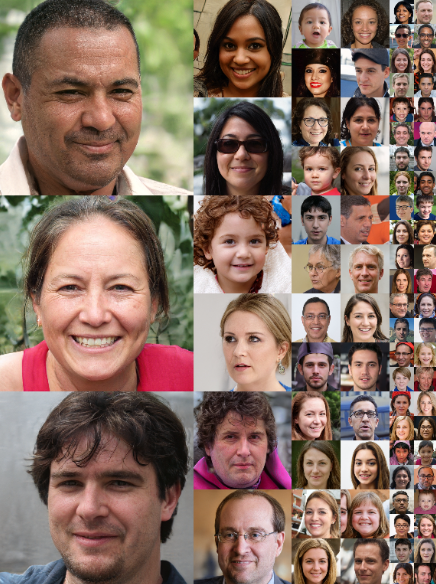
\includegraphics[width=8cm]{resources/styleface.png}
 \captionof{figure}{StyleGAN results}
 \label{fig:style_face}
\end{Figure}

In 2019, NVIDIA's team set out to improve StyleGAN by targeting several of it's characteristic artifacts\cite{DBLP:journals/corr/abs-1912-04958}. In this paper, the team sets out to redesign the generator normalization and regularize the generator to encourage good conditioning in the mapping from latent codes to images. 

To remove normalization artifacts, NVIDIA's team identifies an AdaIN operation that normalizes mean and variance of every feature map sepearately, destroying any information found in the magnitudes of the features relative to each other. They instead remove the normalization step from the generator, causing the droplet artifacts to dissapear.

On the other hand, the generator's architecture is revisited completely. Where the original StyleGAN applies bias and noise within the style block, more predictable results are obtained by their modification, which is moving these operations outside of the style block, operating on normalized data. They also remove the application of bias, noise and normalization to the constant input without any observable drawback in performance or quality.

\subsection{StyleGAN2}
Later in 2020, Karras' team releases the "StyleGAN2" paper \cite{DBLP:journals/corr/abs-2006-06676}. This time around, Karras and his team set out to improve their StyleGAN to work with limited amounts of data. They propose the implementation of an adaptive discriminator augmentation mechanism that stabilizes training when the dataset used is small. They demonstrate that results are not greatly affected even without modifying the loss functions or the architecture of the network.

We tried implementing a variant of the StyleGAN2 for use in our project initially, but our results proved to be too slow, and too poor compared to Karras' team's release. 



\section{Method}
In this section, we will describe the methods used for face and emotion recognition. We also discuss the datasets and propose the methods we will use to make use of them. We propose these methods considering that we need to achieve a minimum viable product for our robot. With this project, we aim to produce a physical prototype, so we have to consider that experimental results will impact the final implementation of the features and how much of a compromise between quality and performance we are willing to make. 



\subsection{FERPlus Dataset}

The FERPlus dataset, published by Barsoum et al. \cite{BarsoumICMI2016}, is an improvement over the previous FER\cite{FER2013} dataset published for a \emph{Kaggle.com} research competition.

FER, prepared by Pierre-Luc Carrier and Aaron Courville. Each image measuring 48 pixels wide and high the dataset consists of ~28k images. The dataset annotations consist of numeric codes ranging from 0 to 6 for the emotion present in the image file: \emph{(0=Angry, 1=Disgust, 2=Fear, 3=Happy, 4=Sad, 5=Surprise, 6=Neutral).}
The FERPlus dataset improves the previous FER dataset by re-tagging the dataset manually\ref{fig:fervsferplus}. FERPlus adds more classes, bringing it up to 8 emotions total. Each image has been labeled by ten independent "taggers" (humans), which means that each face image has a distribution of emotions.



\begin{figure}[h]
  \centering
  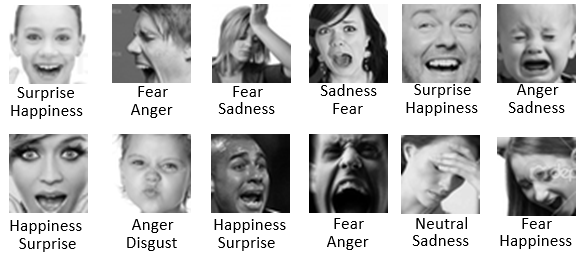
\includegraphics[width=10cm]{resources/fervsferplus.png}
  \caption{Comparison of FER and FERplus labels. Image obtained from the FERPlus paper\cite{BarsoumICMI2016}.}\label{fig:fervsferplus}
\end{figure}


\subsection{COCO 2014 dataset}

Microsoft released their COCO 2014 training dataset as part of a more extensive publication containing training, validation, and test images. Totaling 328K images, it was the largest and most curated dataset at its publication. The dataset contains 80 different classes and multiple captions per image. 


\subsection{Target styles for style transfer}


\begin{figure}[h]
  \centering
  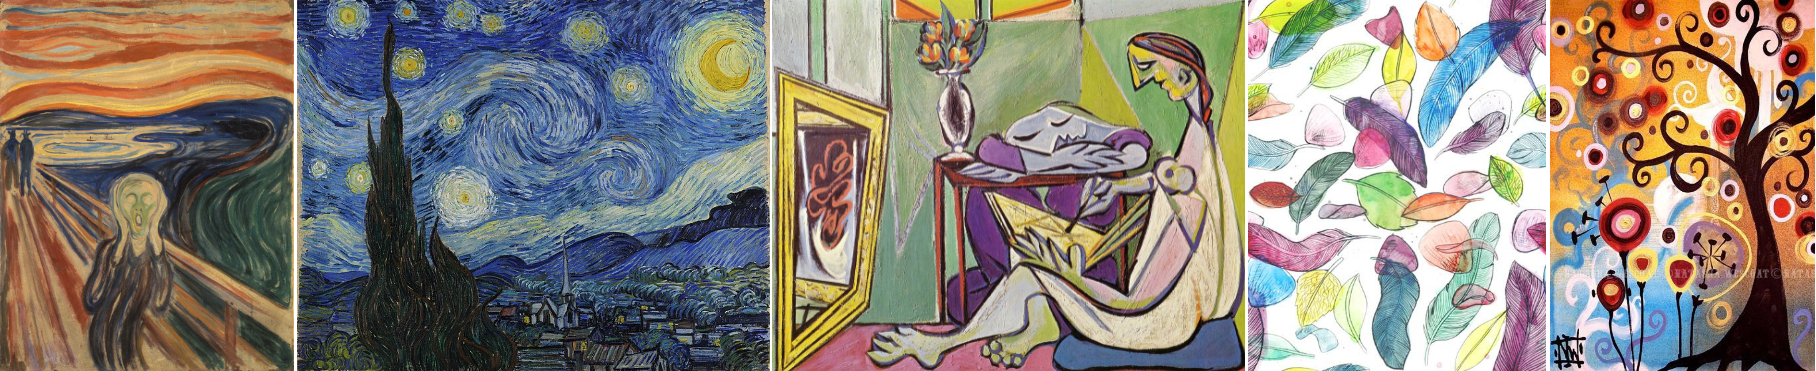
\includegraphics[width = 0.9\textwidth]{resources/target_styles.png}
  \caption{Target Styles. The corresponding assigned emotions, from left to right: Anger, Sadness, Fear, Happiness, Surprise.}
  \label{fig:target_styles}
\end{figure}

We selected five different paintings to be our target styles an assign them an emotion:
         \begin{itemize}
          \item \emph{The Scream} By Edvard Munch\footnote{From: https://www.edvardmunch.org/the-scream.jsp}  for the "anger" emotion, 
          \item \emph{The Starry Night} By Vincent Van Gogh\footnote{From: https://www.vangoghgallery.com/painting/starry-night.html} for the "Sadness" emotion,
          \item \emph{La Musa (Mujer Leyendo)} By Pablo Picasso\footnote{From: https://www.slobidka.com/pablo-picasso/158-picasso-la-musa-mujer-leyendo.html} for the "Fear" emotion,
          \item \emph{Feathers} By Kathryn Corlett\footnote{from: https://www.ebsqart.com/Artist/Natasha-Wescoat/1439/Art-Portfolio/June-Tree/717313/} for the "Hapiness" emotion,
          \item \emph{June tree} By Natasha Wescoat\footnote{From: http://kathryncorlett.blogspot.com/2012/05/wallpaper-feathers-petals-leaves.html} for the "Surprise" emotion.
\end{itemize}

These particular paintings were selected for various reasons. The first, is that some of them are widely used in other style transfer works, so we could compare qualitative results while we were developing them, like \emph{The scream} or \emph{The Starry Night}. We also found some target styles interesting enough to include them, like \emph{Feathers} and \emph{June tree}. 

The emotions assigned to each style were not pre-selected, meaning we did not select a particular style to portray a particular emotion, as the final style transfer image would sometimes not correspond to our pre-selected style. With \emph{The scream}, for instance, logic would have it that it would be selected to represent surprise or fear as that seems to be the motif of the painting, but in our results, we think the black and red hues and aggressive brushstrokes of the style-transferred image confer a more angry emotion rather than the other two.



\subsection{Methodology}
To achieve an MVP (Minimum Viable Product) and be worthy of an MSc project, we set our goals as the following:

\begin{itemize}
  \item Remove the need to use Google's Cloud API for all computer vision tasks, implementing local solutions.
  \item Implement new routines involving engaging computer vision algorithms like Style Transfer.
  \item The user should easily be able to obtain the style transferred files.
  \item The visual representation on the screen should be visually pleasing enough that users will want to keep it on as a background element.
  \item Make the robot completely autonomous: remove the need to offload computation to a 3rd party service or a local machine.
  \item Achieve a real-time representation of the robot's image processing.
\end{itemize}


\subsection{Face detection}

Previously, our pipeline for the robot required sending images to Google's Cloud Services (GCS) for emotion recognition. As we have removed GCS, this is no longer the case. To replace the previous face detection and emotion detection parts of the pipeline, we need to implement local face detection and emotion detection methods based on the current state of the art. Face detection allows the arm to follow a subject should it approach the camera's viewing angle limits. We propose using a Haar-Cascade classifier to detect faces. 

\subsection{Emotion recognition}
Detecting faces in the frame also serves to improve emotion detection. As described in Gunwan et al.\cite{haarcrop}, a neural network trained on cropped faces performs optimally on similarly cropped images. We propose training a network on the FERPlus\cite{BarsoumICMI2016} dataset.


\subsection{Style transfer method proposal}

We will use emotion recognition to change the context of the style transfer network, loosely adapting the target style transfer to a user's visible emotional status.


We propose a local implementation of a neural network capable of producing style transfer images as close to real-time on the Raspberry Pi 4's hardware as possible. The models can be pre-trained in a more powerful environment, but inference should run entirely locally on the device. This way, the robot does not need any external connections or dependencies in run-time. We propose experimenting with two different architectures: a recent model that requires more potent hardware but has better performance (results) and an older model that does not require high-end hardware, producing worse results but potentially giving us faster results and allowing the robot to run inference locally. Thus, we propose adapting Karras' StyleGAN2 representing the "state of the art" method, and since we are already using VGG16 and VGG19 models for our emotion recognition, adapting the method proposed by Justin Johnson et al. on their \emph{"Perceptual Losses for Real-Time Style Transfer
and Super-Resolution"} \cite{Johnson2016Perceptual} publication representing the "old but fast" method to run on our hardware.
While StyleGAN2 was trained using the FFHQ dataset \cite{nvlabs_2019}, we propose using Microsoft's COCO 2014 training dataset\cite{DBLP:journals/corr/LinMBHPRDZ14} to train our style transfer models, as we are not using only face images on our style transfer. 

If one of these two methods can run locally while achieving a good framerate, it should be strongly considered for the final implementation, as it would complete our final two objectives for an MVP.

\subsection{Combining everything to form a product}


We also need a way to get our style transferred images from the robot to the user. We propose using the Telegram Python API, implementing a Telegram bot that users can enable to receive their images on their mobile devices.

When we have all of our methods implemented, we will need a way to create a cohesive user experience through our robot. We need to design and implement a state machine that should conform to the following process:


\begin{enumerate}
  \item User powers the robot on.
  \item Robot searches for faces.
  \item When a face is found, recognize emotion and perform live style transfer.
  \item Whenever the user requests it, provide them with the style-transferred image file.
  \item Whenever the face is lost, go back to state 2)
\end{enumerate}

\section{Experiments}

\begin{itemize}
  \item Fast neural Style: pytorch + vgg19 setup.
  \item Emotion detection: FER
  \item face detection haar cascades
  \item 
\end{itemize}


\subsection{Face and emotion detection}

We used a traditional Haar-Cascade classifier to detect faces within the camera's frame. To test the accuracy and detection rate, we recorded 5 short videos, 400 frames in length each. These frames were used to test the time it took the classifier to produce a result, and the accuracy of these results for our camera's resolution and use-case. 

The features we are looking for in our frames are both faces and eye features, because we not only want to keep a person within the camera's frame, but we also want to pass a cropped photo of the person to the emotion detector, which performs best when both eyes are visible. 

Regarding emotion detection, we used the CNN provided by Octavio Arriaga \cite{DBLP:journals/corr/abs-1710-07557}. On their publication, they report 66\% accuracy on the FER dataset on their "sequential fully-CNN".

When training this on FERPlus, we simplified the number of classes to 5 as we found that the robot's behaviour was too erratic with more classes. Our chosen emotions are happiness, surprise, fear, sadness and anger.


We measure the performance of our face and emotion detection algorithms by how much time it takes for them to produce a result, as each passing frame affects the quality of the final product.

\subsection{Style Transfer}


We started by taking Karras' team StyleGAN2 network description and adapting it to run on the Raspberry Pi 4s hardware. 


The purpose of using Karras' model was to try to minimize the requirements for inference of a trained model following their architecture. Our logic was that minimizing the footprint of the model, inference would be fast enough to complete in real time for our robot. In our early testing, reducing the input images to even below 100 x 100 px produced a model that had an inference time of around 30 seconds per frame on the Raspberry Pi hardware. We decided that the optimizations required to make this model work at a more reasonable speed were outside of our expertise, as we quickly realized that it required a deeper understanding of the Raspberry Pi's hardware to make use of platform-specific instructions. 

We moved onto implementing Justin Johnson's solution on our platform. Jhonson's original publication used Lua with Torch packages to implement a feedforward neural network to improve the speed of the original Gatys et. al paper's results. This implementation takes around 50 milliseconds per frame on a 1200 x 630 pixel image, which seems promising. 

We translated Jhonson's network architecture to be used in Python with Pytorch 1.9. We noticed that, as Jhonson points out in his publication, changing instance normalization for batch normalization has a very sizeable impact on speed performance at the cost of very minimal visual performance, as seen in in an example on figure \ref{fig:norm_comp}. 


\begin{figure}[h]
    \centering
        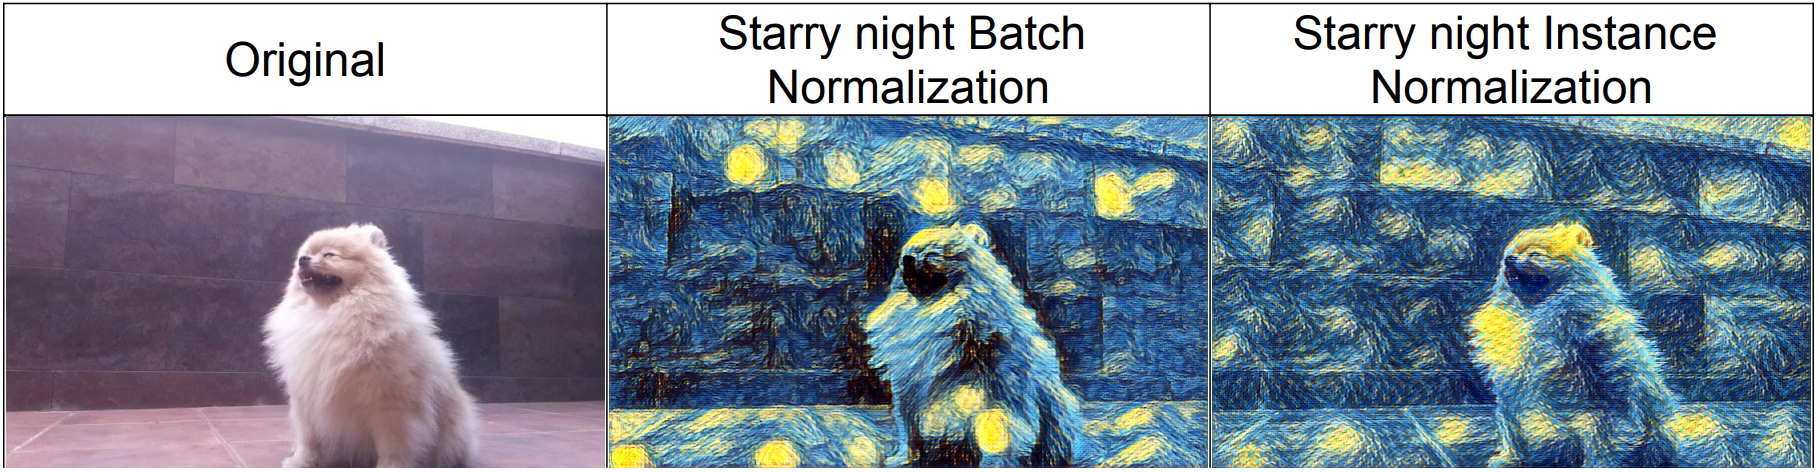
\includegraphics[width=\textwidth]{resources/style_norm_comp.png}        
        \caption{Comparison of instance vs batch normalization}
        \label{fig:norm_comp}
\end{figure}

More importantly, the average processing time for a frame using an instance normalization model was of 1.25 seconds, while batch normalization averaged 0.48 seconds per frame of processing time. 


\begin{figure}[h]
    \centering
        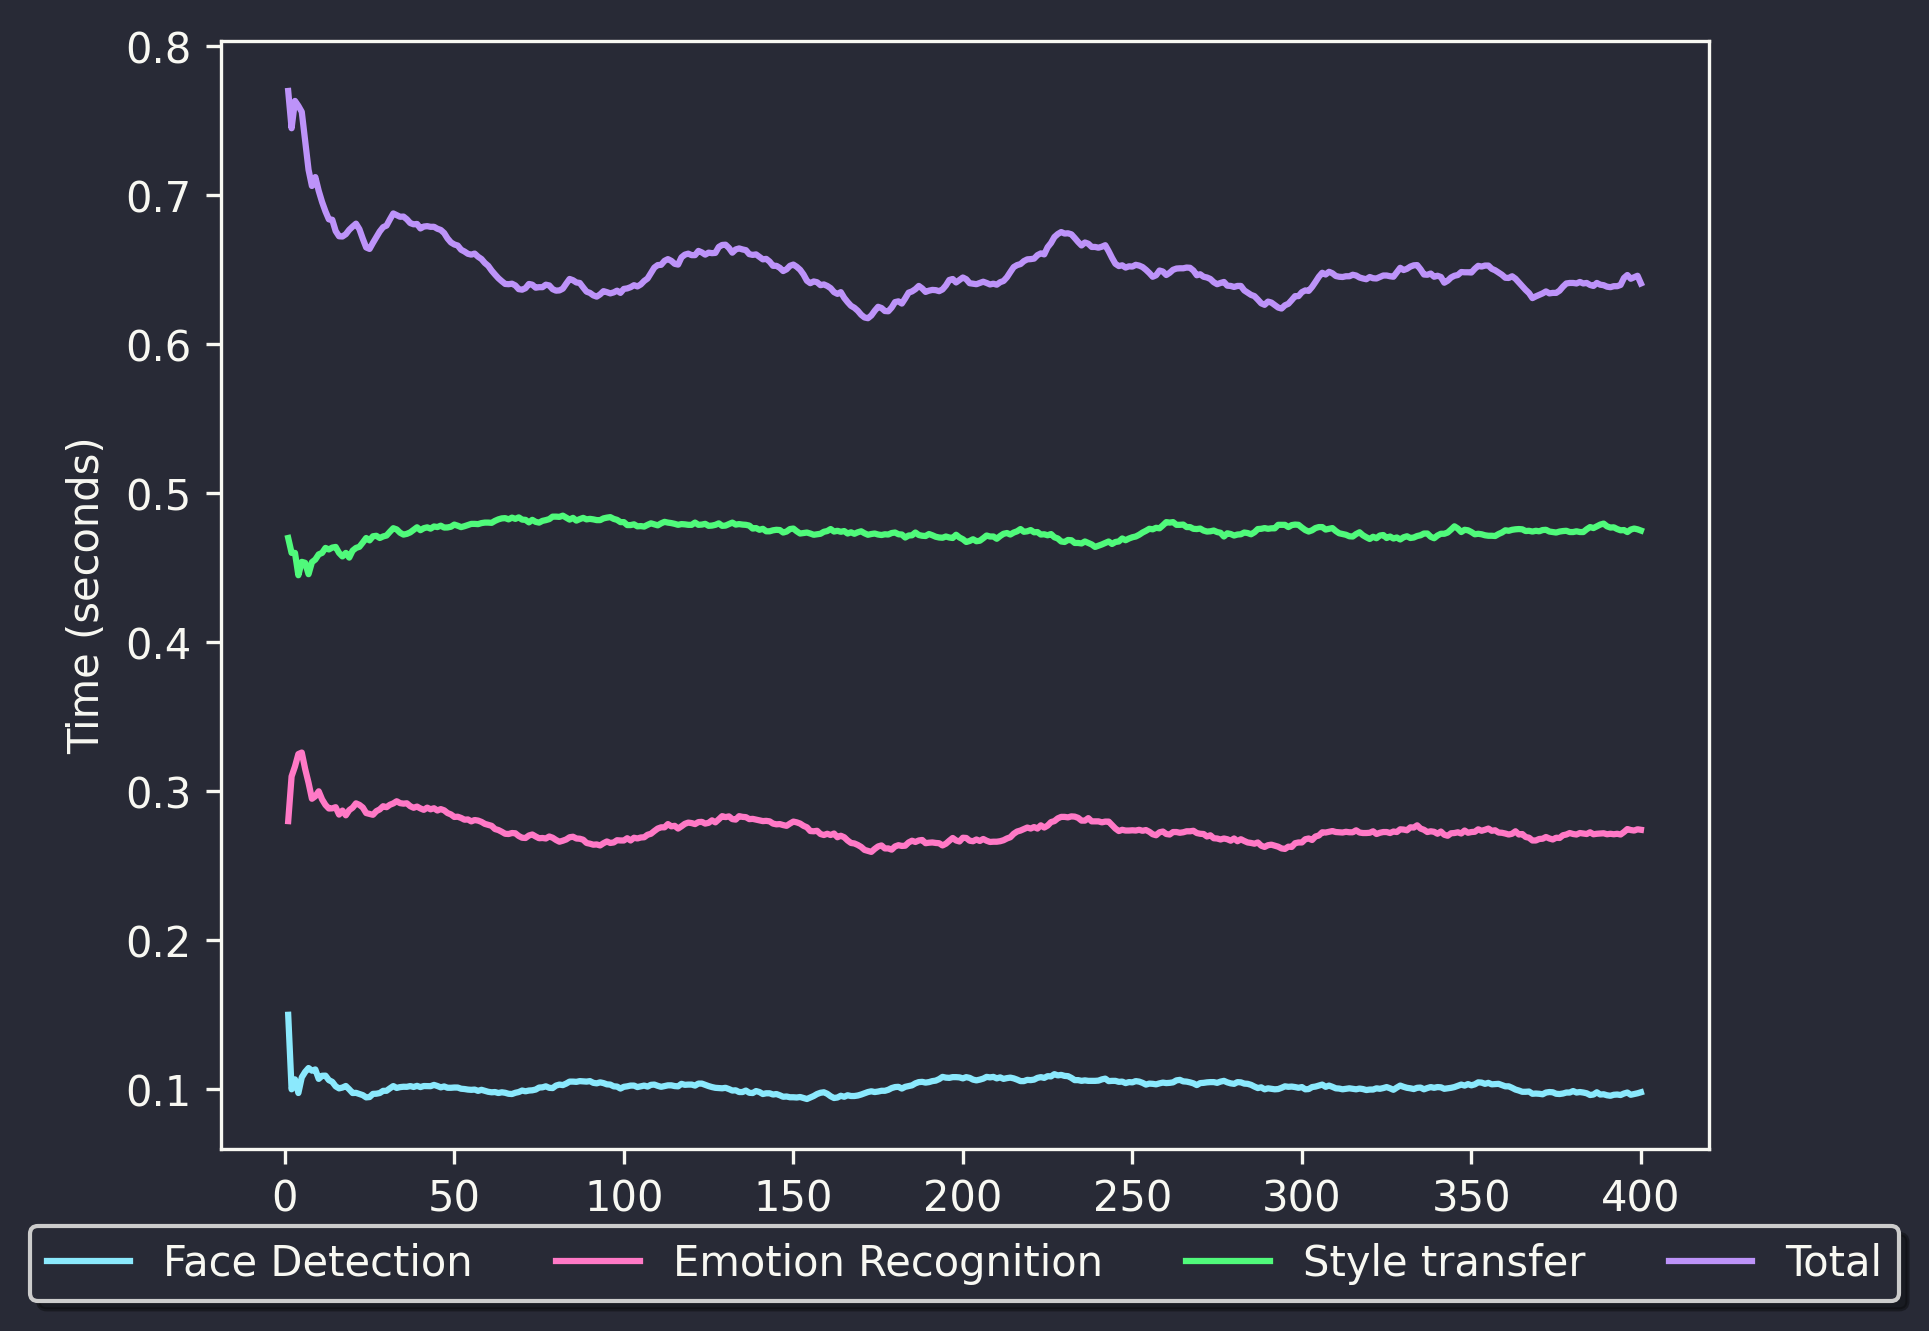
\includegraphics[width=\textwidth]{resources/total_frame_time.png}        
        \caption{Total time consumed per method each frame.}
        \label{fig:total_frame_time}
\end{figure}


\hl{TODO: fast neural style with vgg19}



\subsection{Robot state diagram}

\begin{figure}[h]
  \centering
  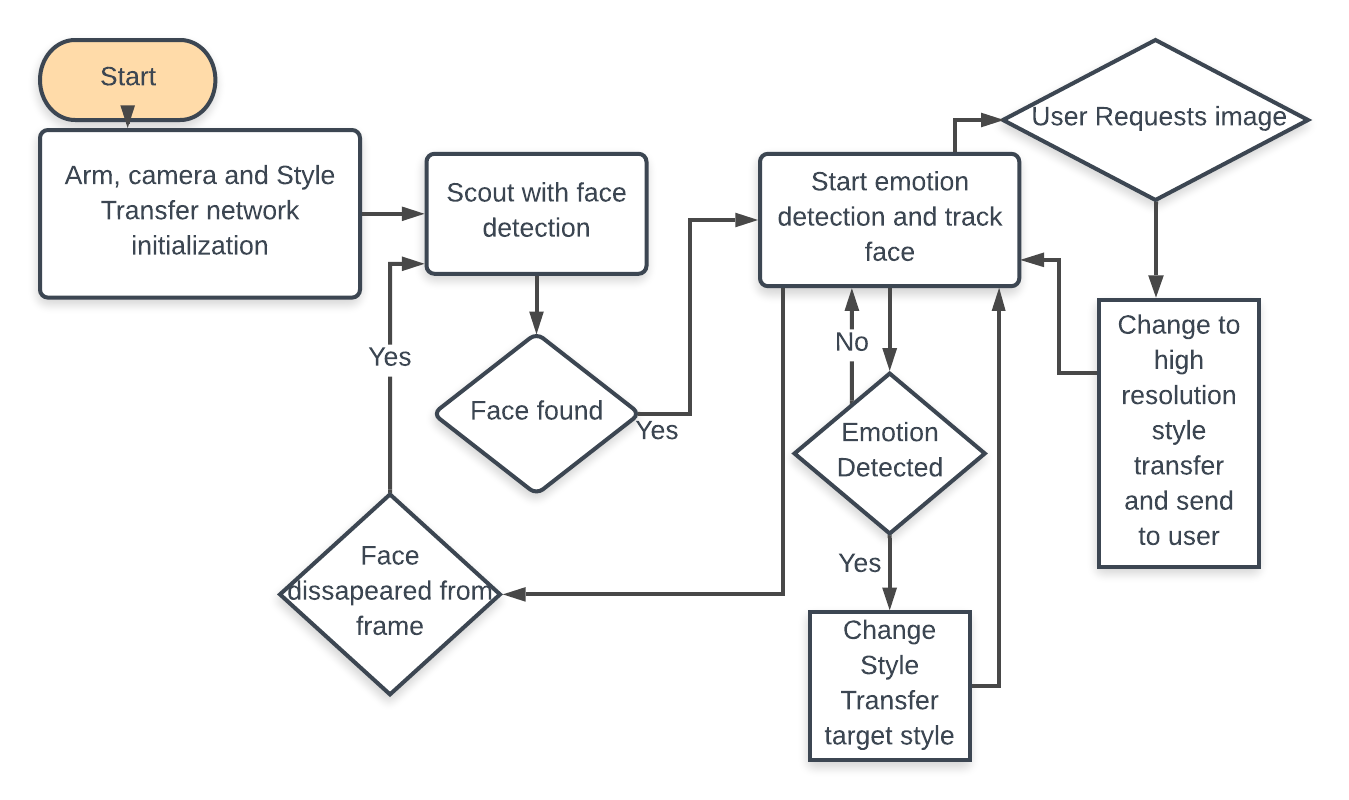
\includegraphics[width=\textwidth]{resources/state_machine.png}
  \caption{Robot flow diagram.}\label{fig:state_machine}
\end{figure}


\section{Results}

In this section, we present the results obtained from our experiments and the performance benchmark, which was the time needed to generate a frame for live-view and the time it took for an image in the high-resolution mode to be processed and sent to the user. We also present qualitative results of the implemented style transferring network and a general overview of the final prototype's functioning.

\subsection{Pre-processing: face and emotion detection}


\begin{figure}[h]
    \centering
    \begin{subfigure}[t]{0.32\textwidth}
        \centering
        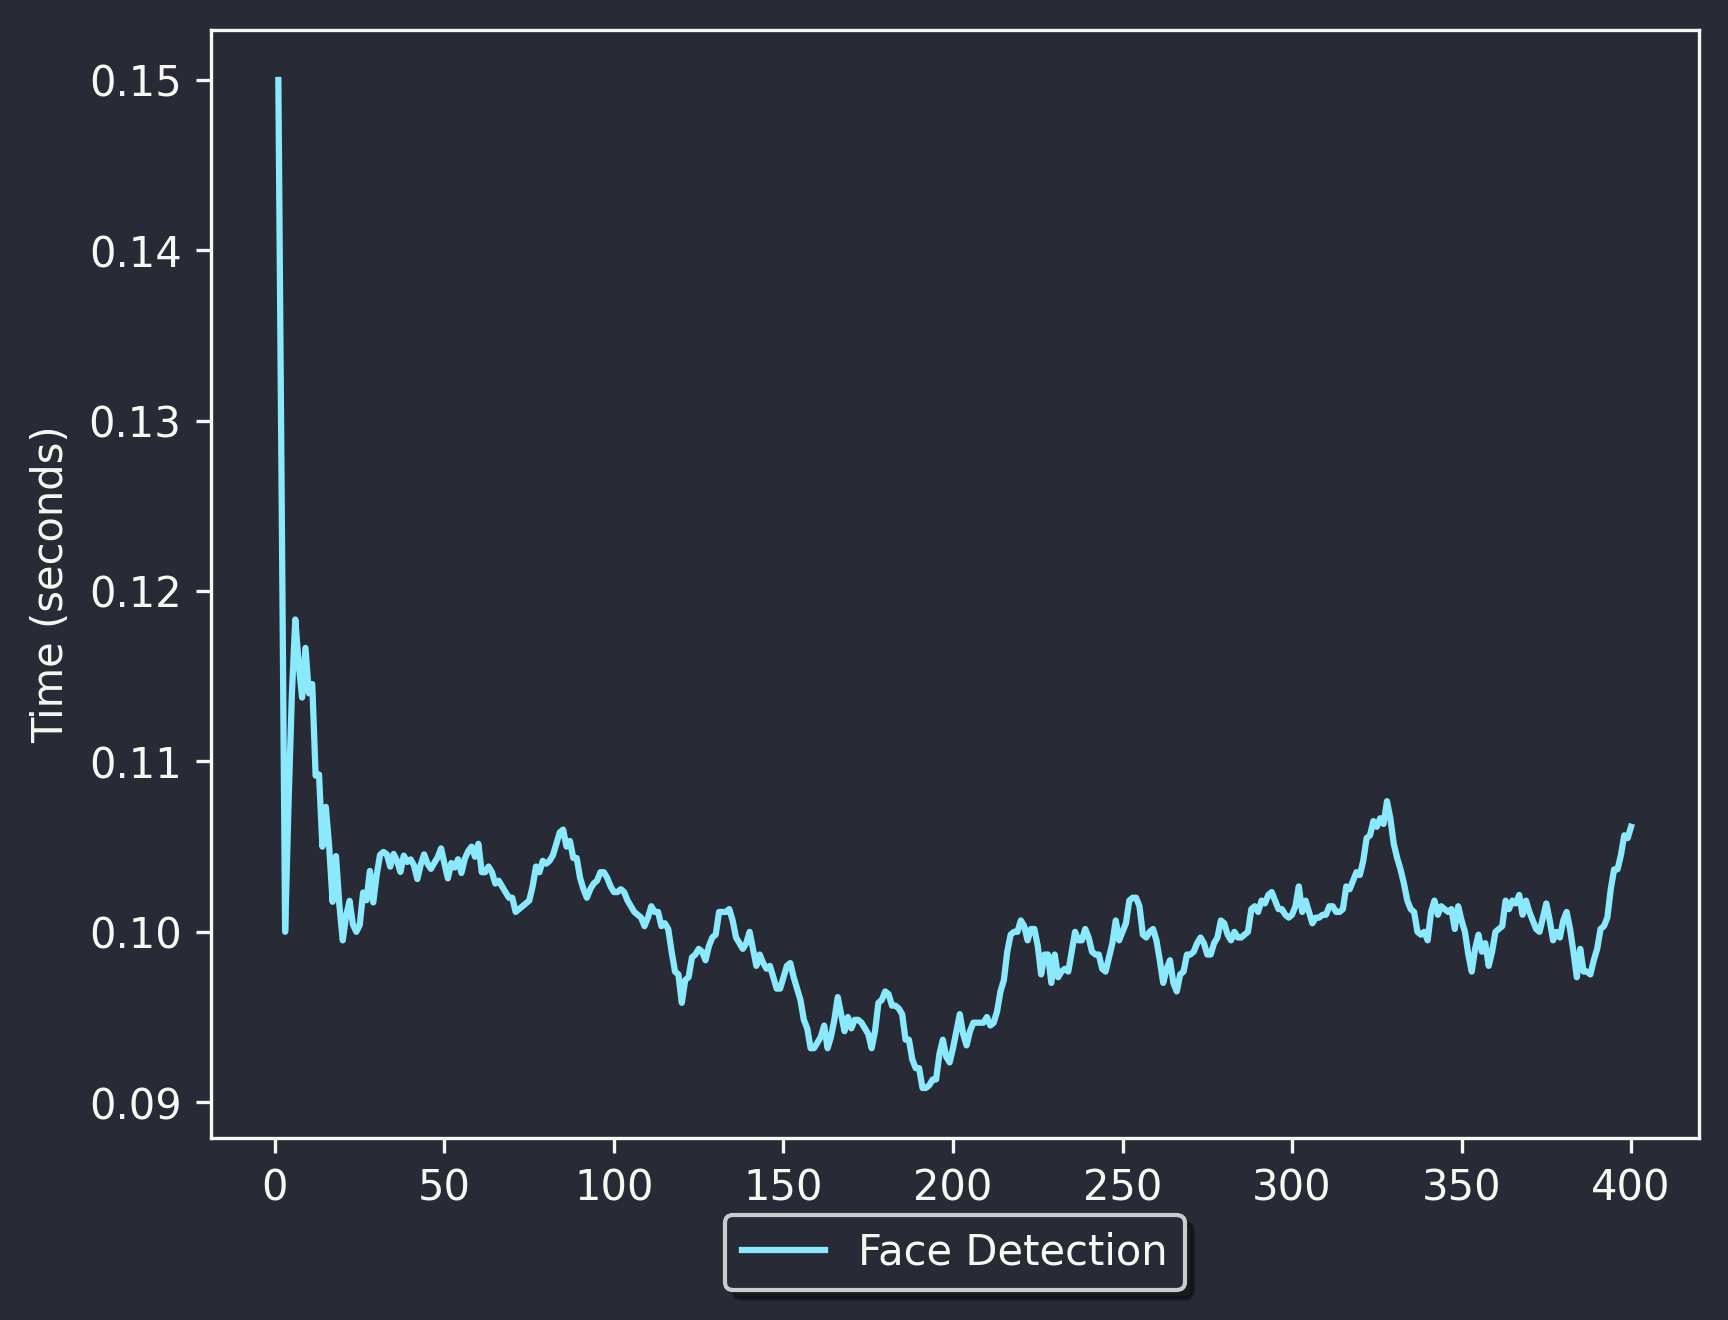
\includegraphics[width = \textwidth]{resources/faceFPS.png}
        \caption{Face detection time per frame.}\label{fig:faceFPS}
    \end{subfigure}
    \begin{subfigure}[t]{0.32\textwidth}
        \centering
        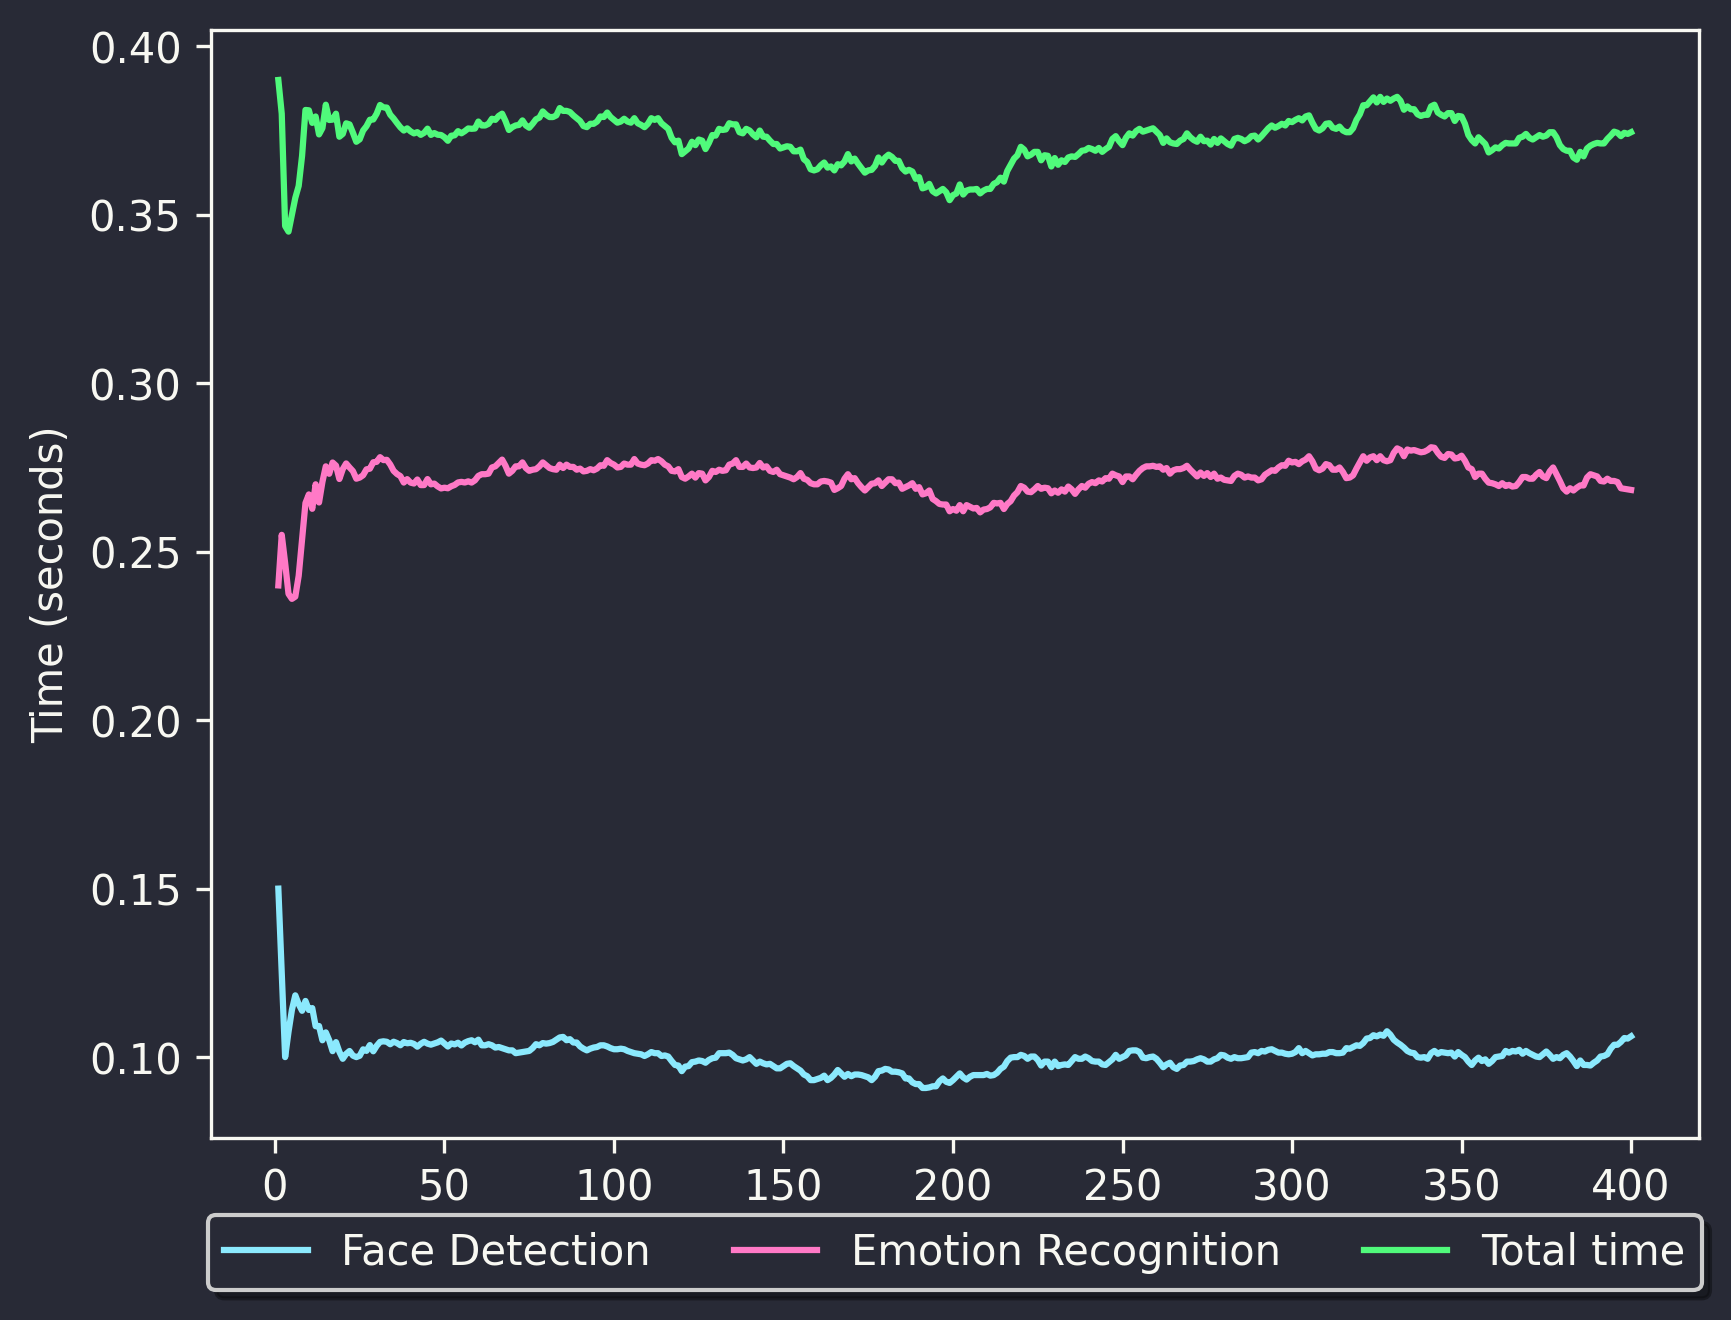
\includegraphics[width = \textwidth]{resources/face_emoFPS.png}
        \caption{Face, emotion detection and total time per frame.}\label{fig:faceemoFPS}
    \end{subfigure}
    \begin{subfigure}[t]{0.32\textwidth}
        \centering
        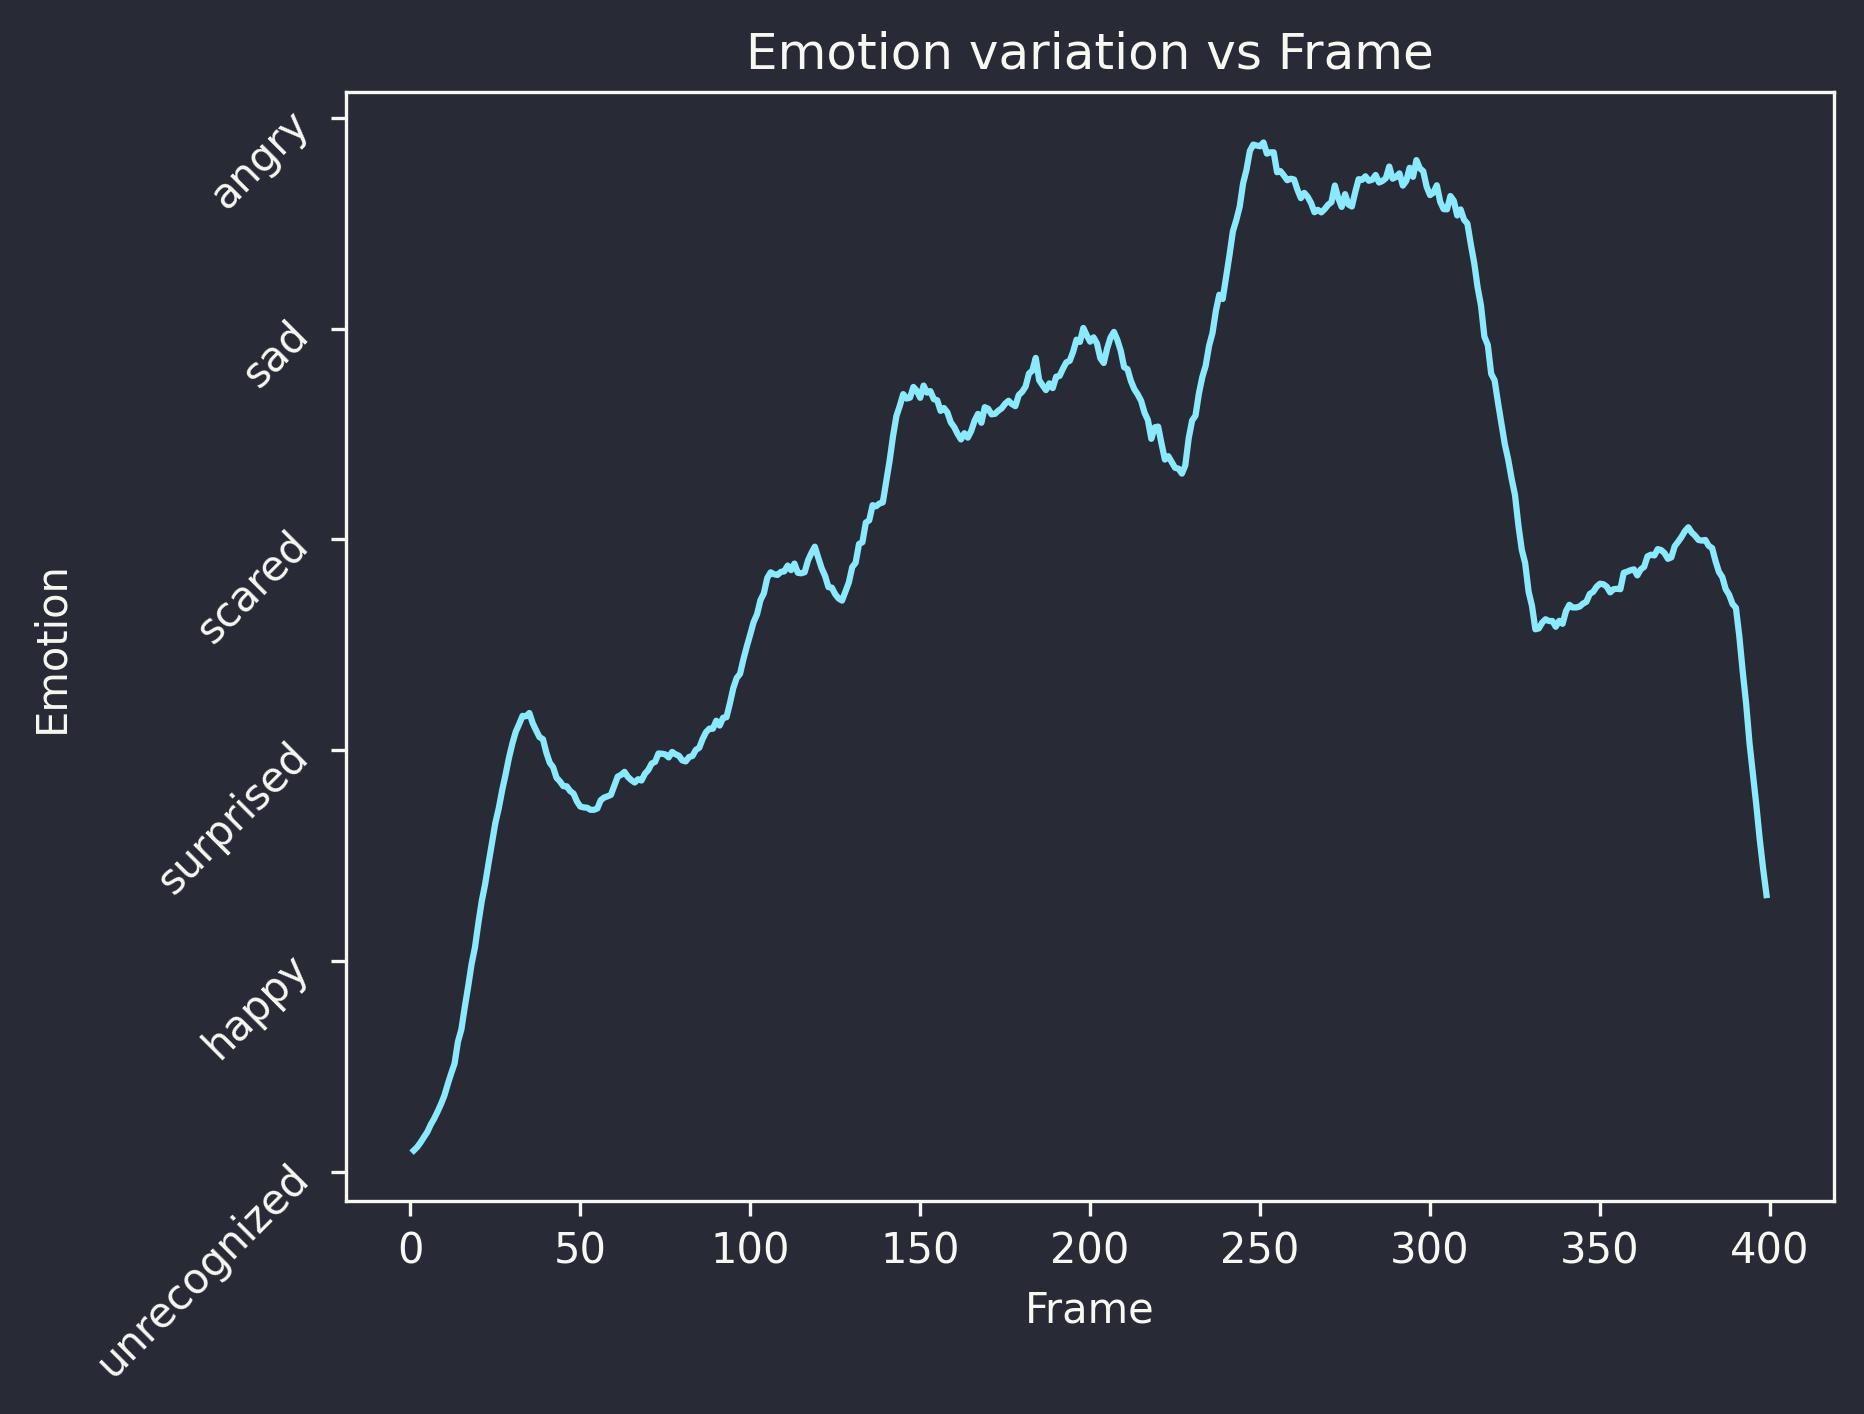
\includegraphics[width = \textwidth]{resources/emotionvsframe.png}
        \caption{Emotion variation by frame of a sample.}\label{fig:emotionvsframe}
    \end{subfigure}
    \caption{Performance of face and emotion recognition.}\label{fig:face_emo_bigtable}
\end{figure}



Our final implementation of face detection can produce results at an average of 0.1 seconds per frame on the Raspberry Pi's hardware, as seen in Figure \ref{fig:faceFPS}.


Our overall performance almost matches the original "sequential fully-CNN" model's performance at 65\% accuracy, but our implementation can complete the recognition of a cropped face's emotion in 0.28 seconds on average, as seen in figure \ref{fig:faceemoFPS}. We also captured a sample for the detected emotion variation for the same sample as our benchmarking run, as seen in figure \ref{fig:emotionvsframe}.


\begin{figure}[h]
    \centering
    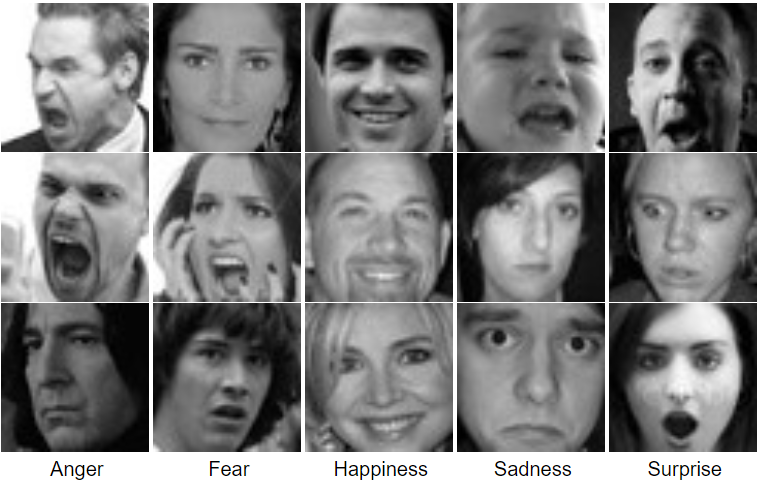
\includegraphics[width = 0.4\textwidth]{resources/emotion_faces_0.png}
    \caption{Emotion detection results sample.}\label{fig:emotion_faces}
\end{figure}



In figure \ref{fig:emotion_faces} you can see a small sample of the performance of our emotion recognition on the FER dataset, and on Table \ref{tab:acc_per_emotion} you can see the performance of the emotion recognition per emotion.

\begin{table}[h]
    \centering
    \begin{tabular}{ll}
        \hline
        \textbf{Emotion}   & \textbf{Accuracy} \\ \hline
        \textbf{Anger}     & 68\%              \\
        \textbf{Sadness}   & 67\%              \\
        \textbf{Fear}      & 60\%              \\
        \textbf{Surprise}  & 64\%              \\
        \textbf{Happiness} & 68\%              \\ \hline
    \end{tabular}
    \caption{Accuracy per emotion}
    \label{tab:acc_per_emotion}
\end{table}

We produced these results by running the network through a subset of images reserved for testing.

\subsection{Style transfer}


As discussed in the experiments section, we implemented StylePi using batch normalization instead of instance normalization. For the most part, this does not affect the quality of the images, but it does ocassionally generate interesting artifacts that produce a clearly different visual result as an effect of batch normalization, as seen in an example on Figure \ref{fig:style_norm_comp}. We believe that this difference, or "pattern-ization" of the image is the product of how batch normalization works, as we can see in the same figure how the "swirling" pattern of Van Gogh's starry night repeats itself in a regular manner. It is not clear to the author under what conditions this happens, as all models have exhibited this behaviour at some point of the experimental phase.


\begin{figure}[h]
    \centering
    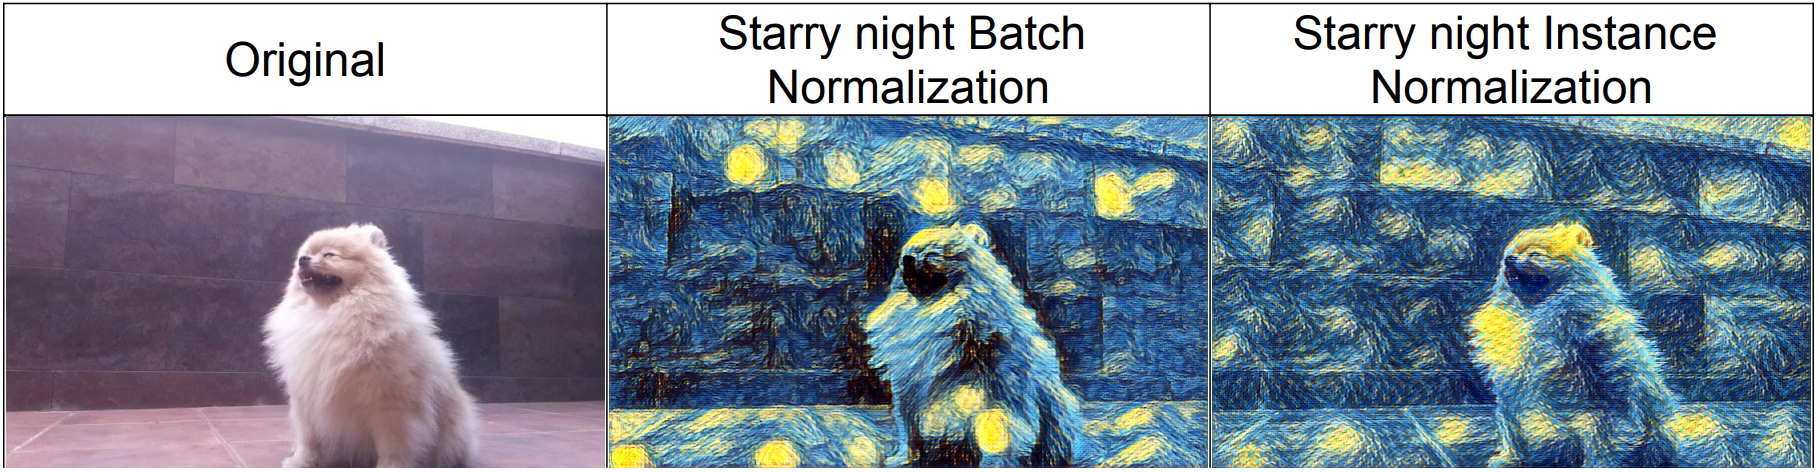
\includegraphics[width = 0.9\textwidth]{resources/style_norm_comp.png}
    \caption{Comparison of instance vs batch normalization}
    \label{fig:style_norm_comp}
\end{figure}

Ultimately, however, batch normalization was able to provide an average processing time of 0.47 seconds per frame over a 400 frame sample, as seen in Figure \ref{fig:finalFPS}.

\begin{figure}[h]
    \centering
    \begin{subfigure}[t]{0.45\textwidth}
        \centering
        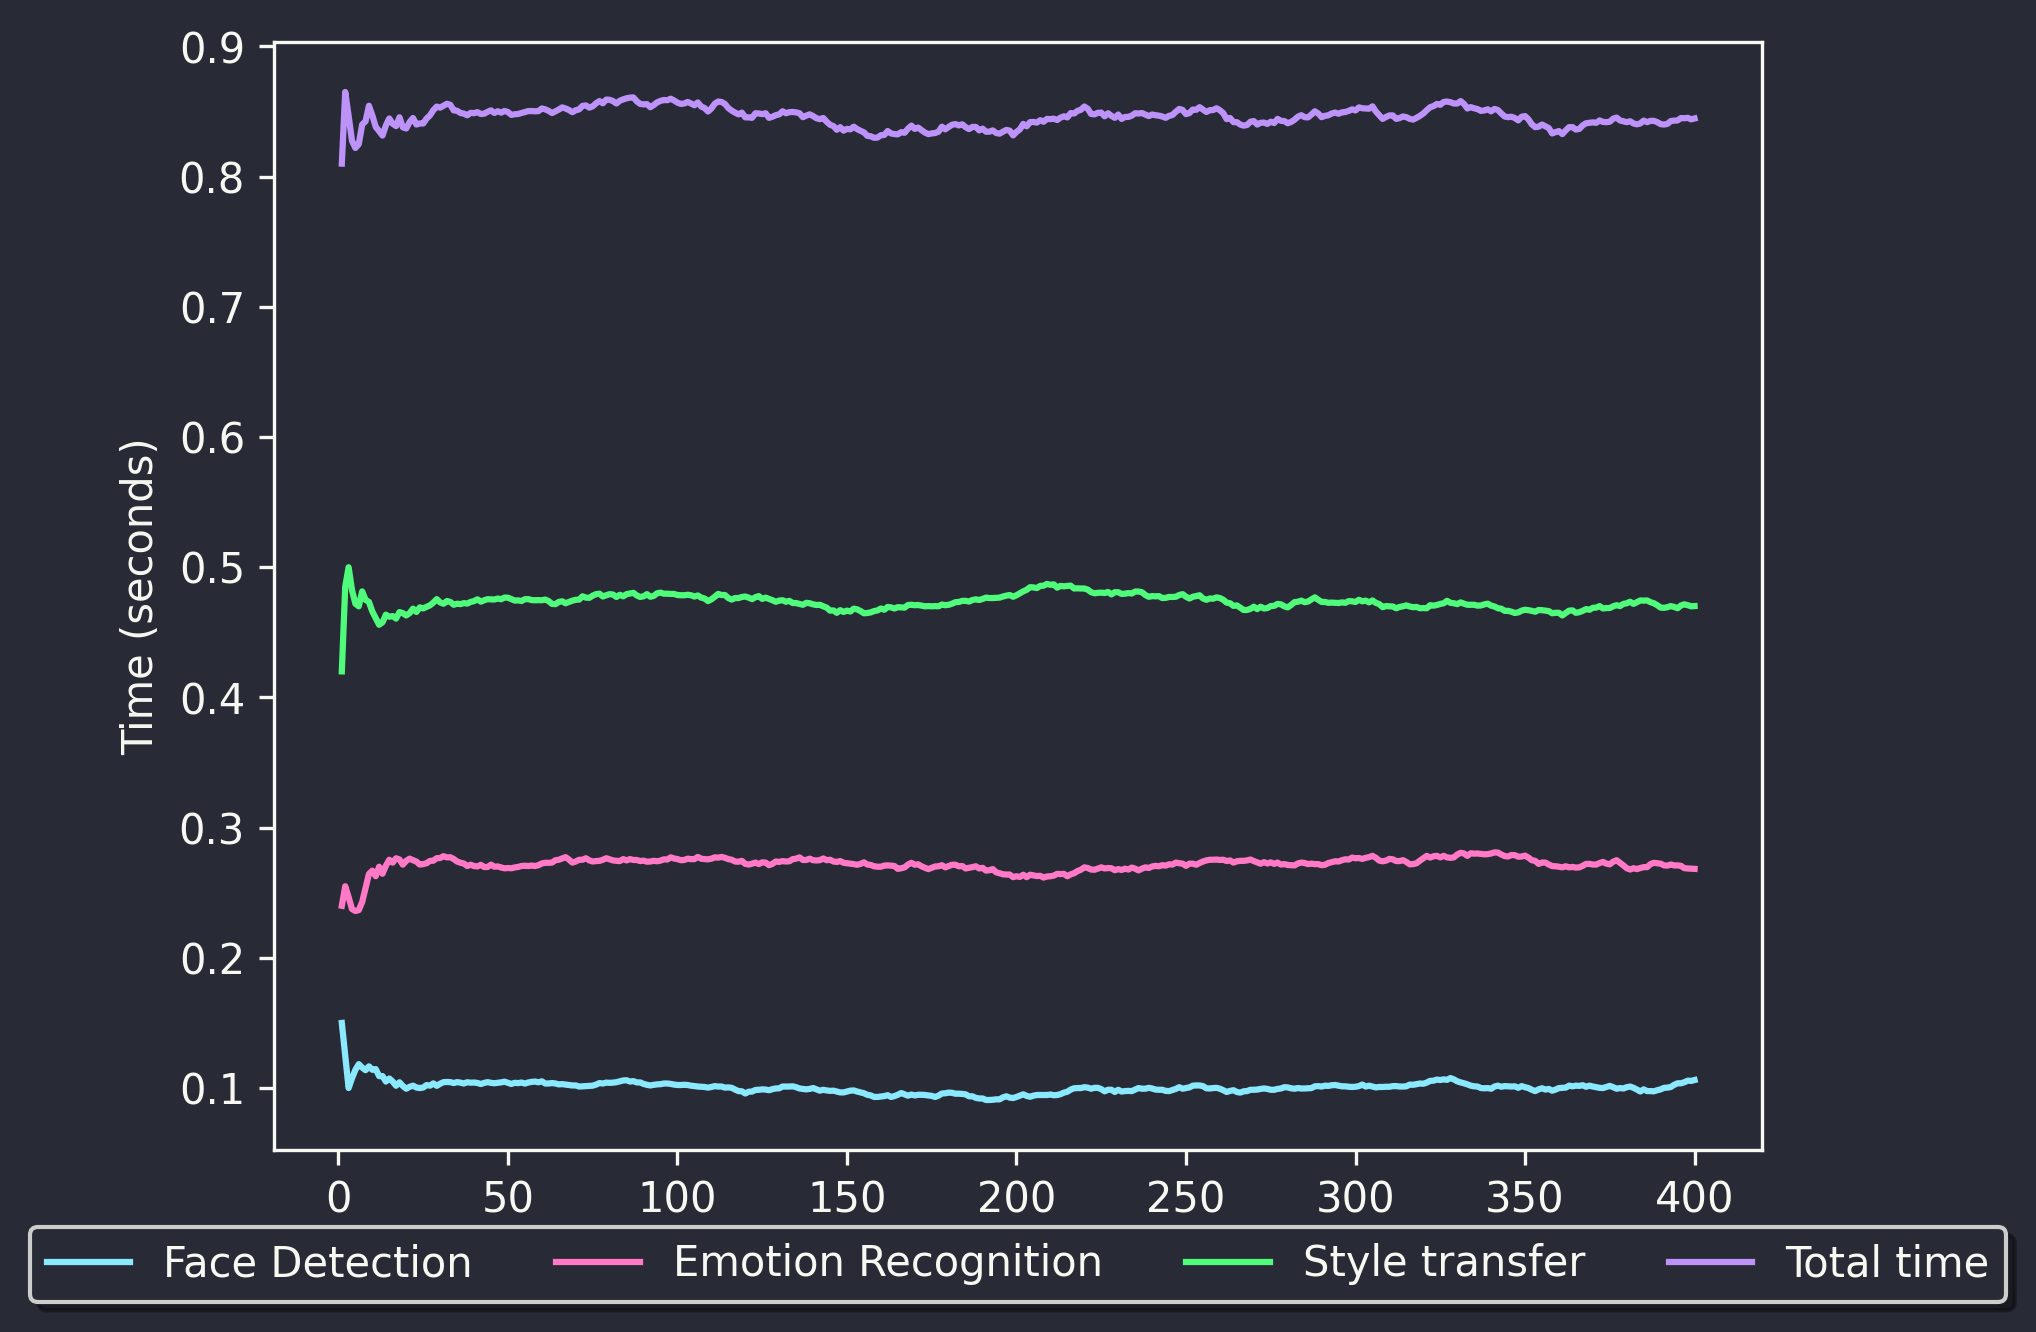
\includegraphics[height = 5.3cm]{resources/finalFPS.png}
        \caption{Performance of face/emotion detection and style transfer per frame.}\label{fig:finalFPS}
    \end{subfigure}
    \begin{subfigure}[t]{0.45\textwidth}
        \centering
        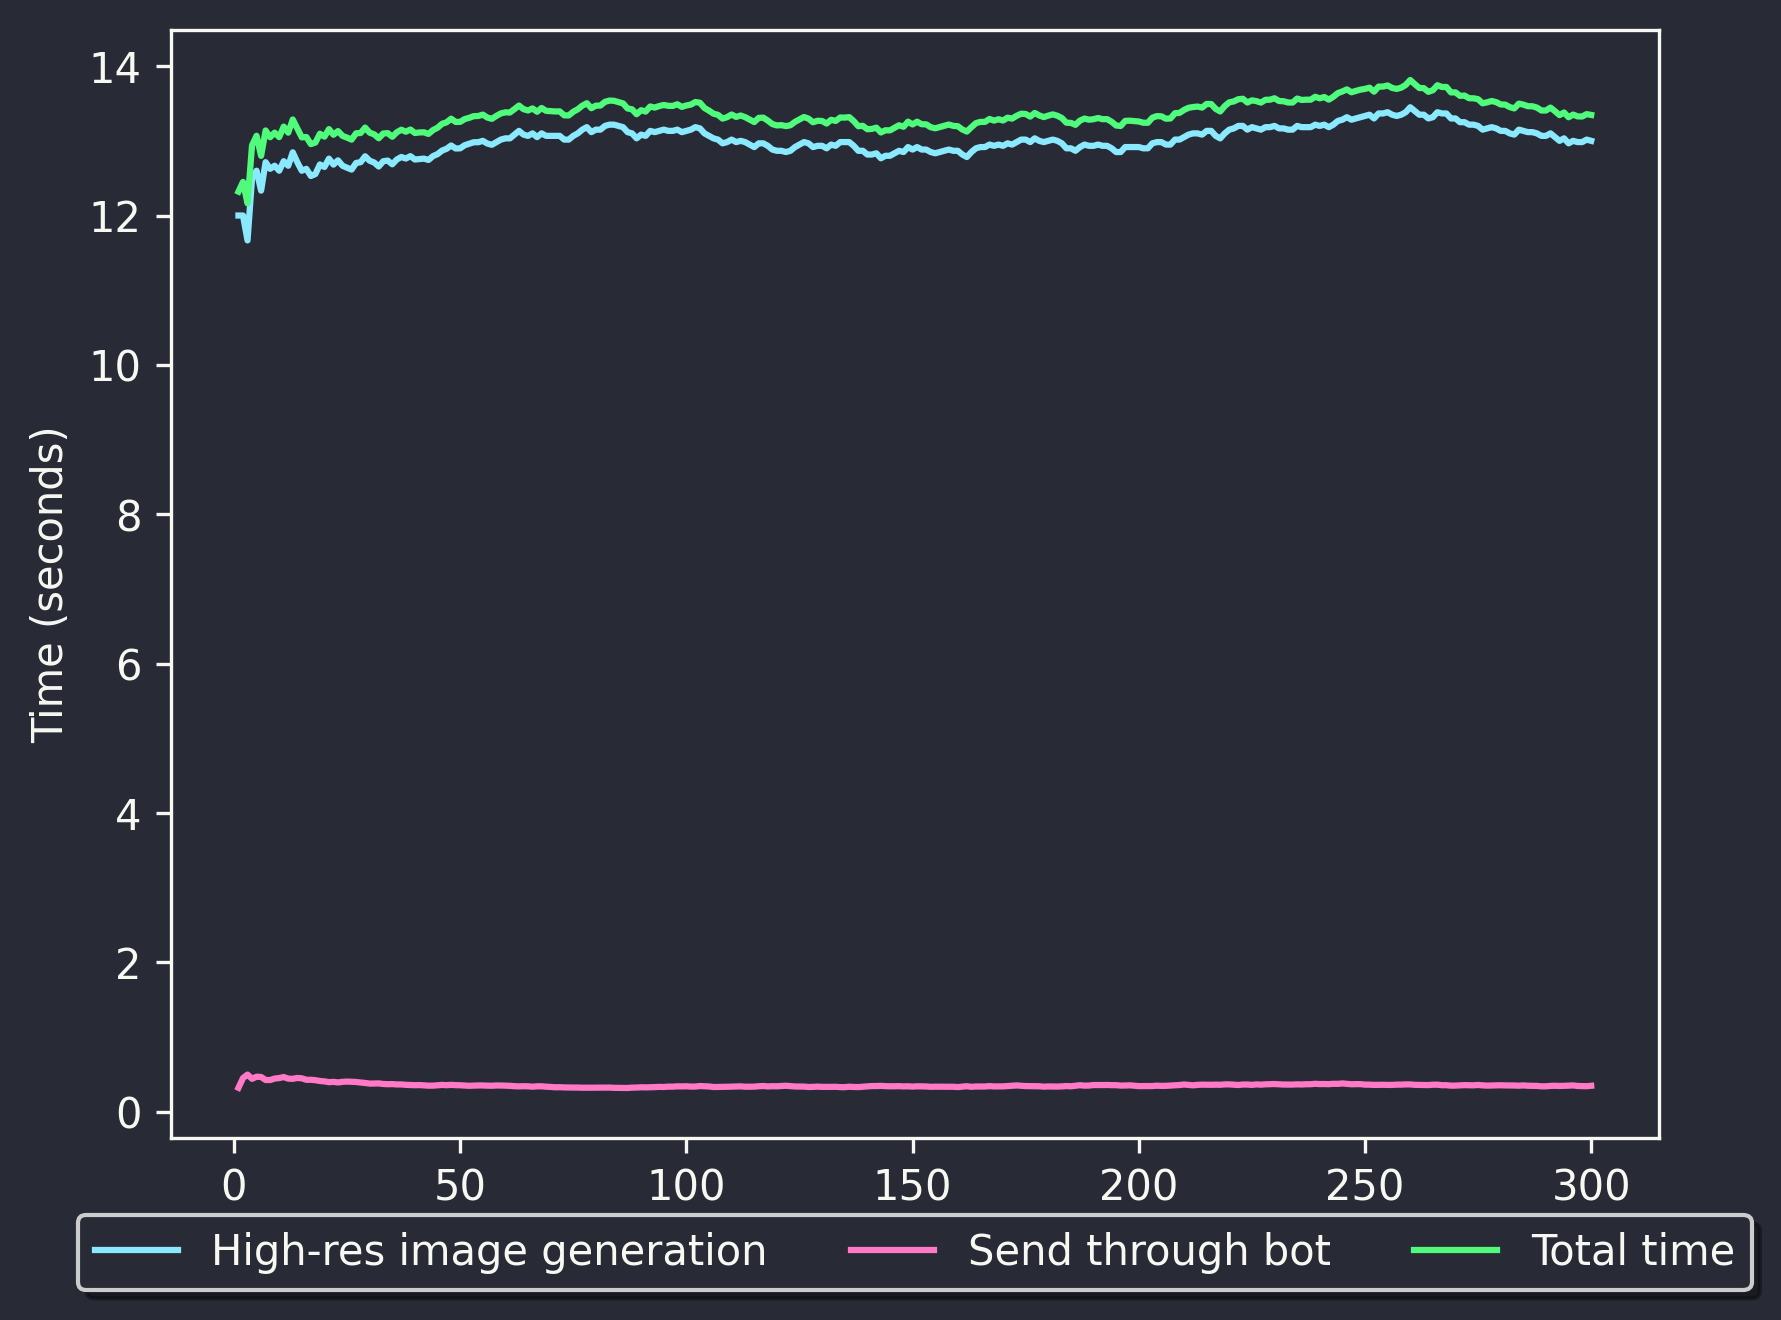
\includegraphics[height =5.3cm]{resources/result_generation_time.png}
        \caption{Total time needed to generate a high resolution image and send it through the bot.}
        \label{fig:result_generation_time}
    \end{subfigure}
    \caption{Final performance per frame and time needed to generate high-resolution images.}\label{fig:final_results_big_fig}
\end{figure}

\subsection{Final MVP performance}

In figure \ref{fig:style_results_grid} you can see the available styles and their associated emotions for a sample image. This figure also includes the output of both modes of the StylePi network: a high resolution and a low-resolution output.

\begin{figure}[h]
    \centering
    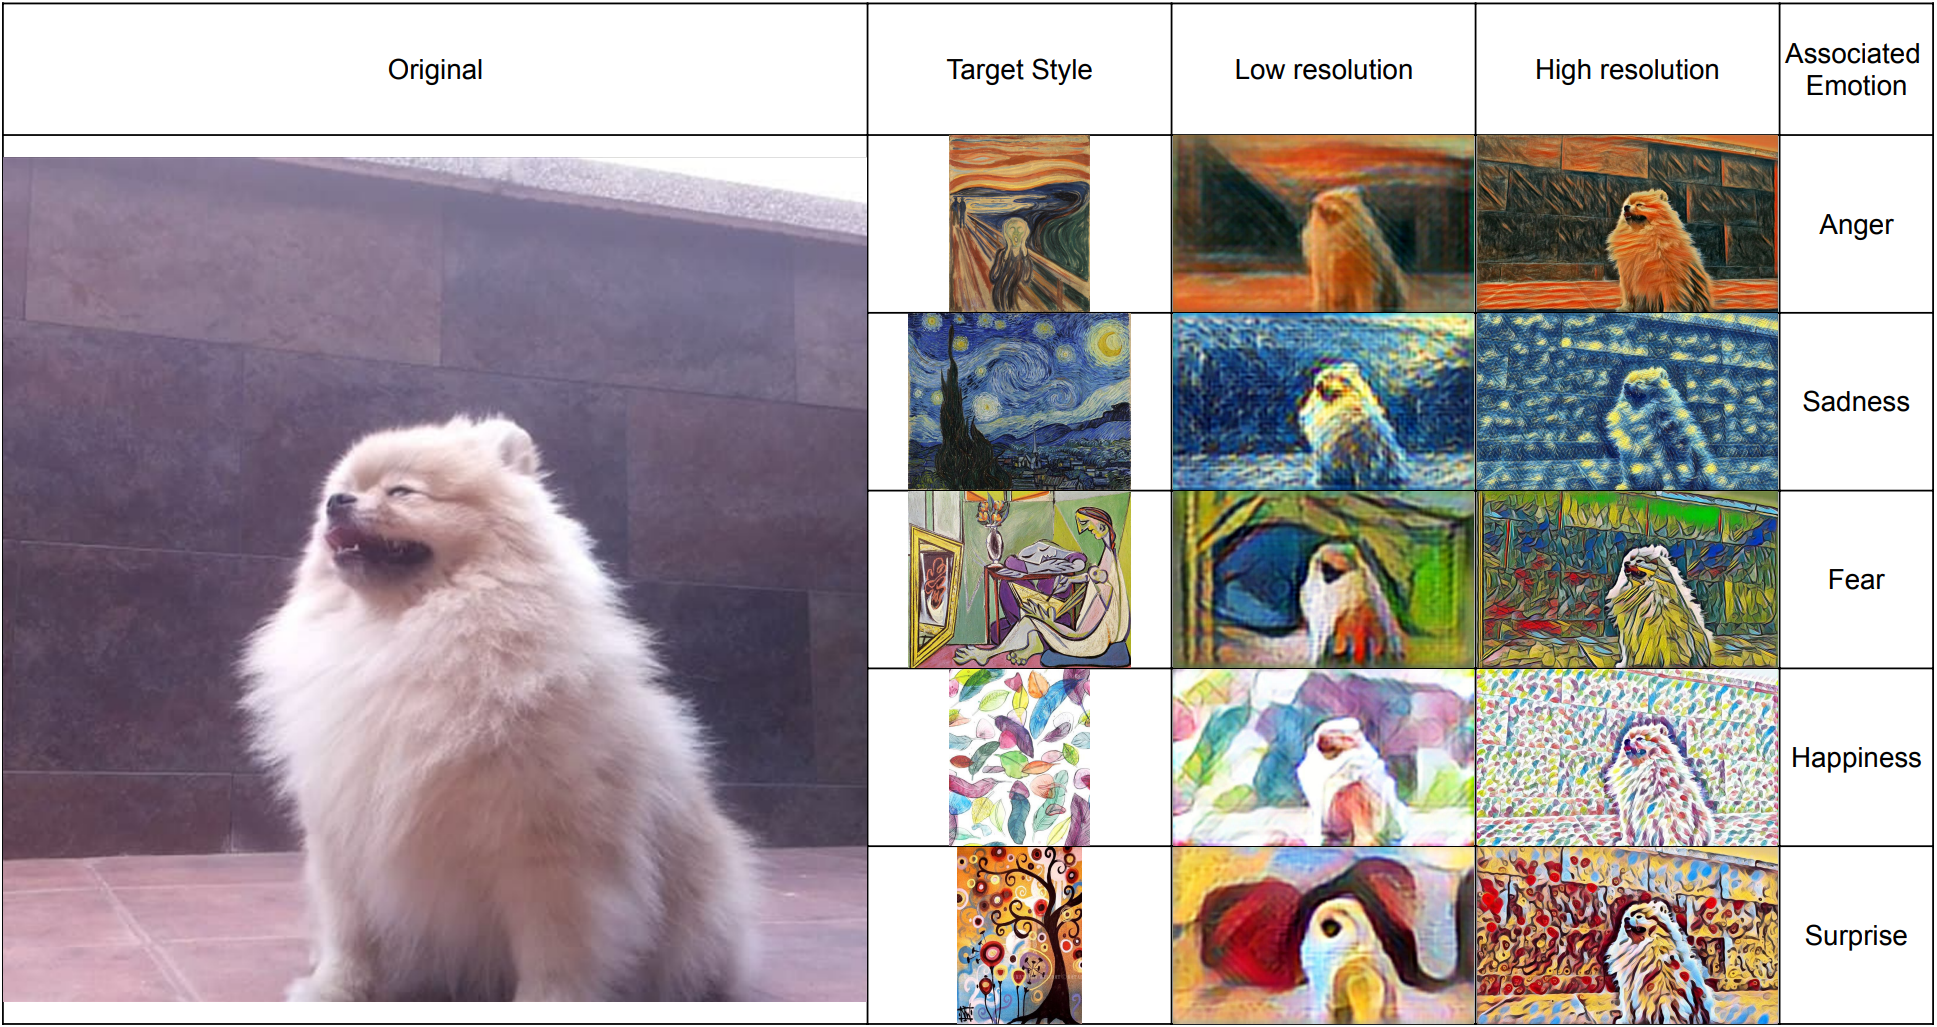
\includegraphics[width = \textwidth]{resources/styletransfer_emogrid.png}
    \caption{Available style transfers for emotion context switching sample. From top to bottom:
        \emph{The scream} By Edvard Munch,
        \emph{The Starry Night} By Vincent Van Gogh,
        \emph{La Musa (Mujer Leyendo)} By Pablo Picasso,
        \emph{Feathers} By Kathryn Corlett,
        \emph{June tree} By Natasha wescoat.
    } \label{fig:style_results_grid}
\end{figure}
The user can request all images generated by the MVP through the provided Telegram bot. The average time needed to generate a high-resolution style transfer of the camera's captured frame and send it through the telegram bot to the user can be seen in Figure \ref{fig:result_generation_time}. We found that selecting the minimum number of images (one) vs. selecting the maximum number of images (five: Original, Lowres, Lowres upscaled, Highres, Highres upscaled) did not impact the time it takes for the bot to send them.


\section{Conclusions}

In this section, we discuss what we achieved and the conclusions of the project. 

The initial goal of this thesis was to create a physical proof of concept that implements computer vision algorithms to aid in interaction in the form of a self-built robotic arm with a camera. This robot's purpose was to allow users to easily interact with computer vision processes like style transfer for story-telling and publication on social media.

In this Computer Vision Master's thesis, we have implemented several computer vision methods using machine learning and traditional methods on a physical prototype capable of functioning in real-time. We have produced a physical prototype at the MVP stage of development with all initial objectives accomplished.
We have adapted face and emotion recognition that works in real-time on the Raspberry Pi's hardware.

Even though we failed at adapting a Generative Adversarial Network to run inference at a reasonably fast framerate on the Raspberry Pi's hardware, we finalized a style transfer feedforward neural network that works on it in real-time.  

We have also integrated our methods into a cohesive software and hardware package that can serve results to the end-user in a fast and effective manner, without relying on external services to perform its primary functions.


\section{Future work}

In this last section, we would like to introduce a short discussion about future improvements and the next steps needed to improve the quality of the MVP. 

We believe that the StylePi network is capable of producing results at a faster rate. A deeper understanding of the Raspberry Pi architecture and the use of a 64-bit OS instead of the public, stable release of Raspbian OS 32-bit used in this project should allow for a modest boost in performance for both framerate and resolution of the images in the "low resolution" mode.
Our feedforward architecture based on VGG19 is not the only method to implement a neural network that can work in real-time on this hardware. A deeper understanding of our target platform and more experience designing and training neural networks should also result in better performance for our robot.

We also wish we could have had implemented a way to record and style transfer a video using this prototype, but our implementation did not allow us to do so without turning off the live-view feature of the low-resolution style transfer mode.

After going through a few test cycles and having other users use the robot, we realized we had a few oversights in the design decisions for the interface. A Telegram bot and directly accessing the Raspberry Pi's storage should not be the only ways to access the produced images. We propose other methods with familiar third parties like Google and Apple account log-in, allowing users to upload the generated images to their services. 


\clearpage
\appendices
\section{Appendix title}
Appendix one text goes here.


% use section* for acknowledgement
\section*{Acknowledgment}


The authors would like to thank...


% Can use something like this to put references on a page
% by themselves when using endfloat and the captionsoff option.
\ifCLASSOPTIONcaptionsoff
  \newpage
\fi



% trigger a \newpage just before the given reference
% number - used to balance the columns on the last page
% adjust value as needed - may need to be readjusted if
% the document is modified later
%\IEEEtriggeratref{8}
% The "triggered" command can be changed if desired:
%\IEEEtriggercmd{\enlargethispage{-5in}}

% references section

% can use a bibliography generated by BibTeX as a .bbl file
% BibTeX documentation can be easily obtained at:
% http://www.ctan.org/tex-archive/biblio/bibtex/contrib/doc/
% The IEEEtran BibTeX style support page is at:
% http://www.michaelshell.org/tex/ieeetran/bibtex/
%\bibliographystyle{IEEEtran}
% argument is your BibTeX string definitions and bibliography database(s)
%\bibliography{IEEEabrv,../bib/paper}
%
% <OR> manually copy in the resultant .bbl file
% set second argument of \begin to the number of references
% (used to reserve space for the reference number labels box)

\medskip

\bibliographystyle{IEEEtran}
\bibliography{references.bib}


% biography section
% 
% If you have an EPS/PDF photo (graphicx package needed) extra braces are
% needed around the contents of the optional argument to biography to prevent
% the LaTeX parser from getting confused when it sees the complicated
% \includegraphics command within an optional argument. (You could create
% your own custom macro containing the \includegraphics command to make things
% simpler here.)
%\begin{IEEEbiography}
%    [{\includegraphics[width=1in,height=1.25in,clip,keepaspectratio]{mshell}}]{Michael Shell}
% or if you just want to reserve a space for a photo:

% You can push biographies down or up by placing
% a \vfill before or after them. The appropriate
% use of \vfill depends on what kind of text is
% on the last page and whether or not the columns
% are being equalized.

%\vfill

% Can be used to pull up biographies so that the bottom of the last one
% is flush with the other column.
%\enlargethispage{-5in}



% that's all folks
\end{document}


